\chapter{Items and Equipment}

This chapter defines the items and equipment that exist in the universe of Rise, including both magical and nonmagical items.
Items are divided into five broad categories, described below.
\begin{itemize}
    \item Weapons are typically used to make \glossterm{strikes}.
        Weapons come in many forms, and can have very different uses in combat.
    \item Armor is worn or wielded to protect yourself.
        There are two types of armor: body armor and shields.
    \item Apparel items are worn on the body, but unlike armor they have no intrinsic defensive properties.
        Rings, cloaks, and all manner of other worn items are considered apparel.
        The only mechanically significant apparel items are \magical.
    \item Implements are typically held while casting spells or using other magical abilities.
        The only mechanically significant implements are \magical.
    \item Tools are used to achieve an effect instead of worn on the body.
        Potions, traps, and magic bags are all tools.
\end{itemize}

\section{Wealth And Item Ranks}\label{Wealth}\label{Wealth and Item Ranks}

    The worth of an item can be measured with money, or with the more abstract concept of an item's rank.
    Both measurements are closely connected.
    In general, gold pieces are a more useful concept at low levels, and item rank are more useful at high levels.
    However, both concepts function at any level, so you can use whichever makes more sense in a particular game.

    \subsection{Coins}
        The most common coin is the gold piece (gp). A gold piece is worth 10 silver pieces. Each silver piece is worth 10 copper pieces (cp). In addition to copper, silver, and gold coins, there are also platinum pieces (pp), which are each worth 10 gp.

        The standard coin weighs about a third of an ounce (fifty to the pound).

        \begin{dtable}
            \lcaption{Coin Exchange Values}
            \begin{dtabularx}{\columnwidth}{l c *{4}{>{\ccol}X}}
                                    &   & \tb{CP} & \tb{SP} & \tb{GP} & \tb{PP} \tableheaderrule
                Copper piece (cp)   & = & 1       & 1/10    & 1/100   & 1/1,000 \\
                Silver piece (sp)   & = & 10      & 1       & 1/10    & 1/100   \\
                Gold piece (gp)     & = & 100     & 10      & 1       & 1/10    \\
                Platinum piece (pp) & = & 1,000   & 100     & 10      & 1
            \end{dtabularx}
        \end{dtable}

    \subsection{Item Ranks}\label{Item Ranks}

        Each item has a rank associated with it.
        An item's rank is generally correlated with the item's effectiveness, rarity, and value.
        A magic item's \glossterm{power} is equal to the class bonus to power that a barbarian of that rank would have.
        These effects are summarized in \trefnp{Item Ranks}.

        In general, five items of a given rank are worth the same as a single item that is one rank higher.
        Likewise, one item of a given rank is worth four items that are each one rank lower.

        \parhead{Gear and Consumables}
            Long-term items that are expected to be worn or otherwise used repeatedly are more expensive than items that are destroyed immediately after being used.
            Although consumable items are cheaper, they still use their full rank for all other purposes, such as their power and how difficult they are to buy.
            In general, five consumable items of a given rank are worth as much as a single non-consumable item of that rank.

        \begin{dtable}
            \lcaption{Item Ranks}
            \begin{dtabularx}{\columnwidth}{l l X X}
                \tb{Rank} & \tb{Power} & \tb{Typical Gear Price} & \tb{Typical Consumable Price} \tableheaderrule
                0 & 2 & 10 gp or less & 2 gp or less \\
                1 & 3 & 40 gp         & 8 gp         \\
                2 & 4 & 200 gp        & 40 gp        \\
                3 & 5 & 1,000 gp      & 200 gp       \\
                4 & 7 & 5,000 gp      & 1,000 gp     \\
                5 & 10 & 25,000 gp     & 5,000 gp     \\
                6 & 14 & 125,000 gp    & 25,000 gp    \\
                7 & 20 & 625,000 gp    & 125,000 gp   \\
            \end{dtabularx}
        \end{dtable}

        Items with a rank of 0 or 1 may be found among common folk, though few commoners would have more than one magic item of any value.
        Items with a rank of 2 or higher are usually only owned or used by nobility, wealthy merchants, and adventurers.

    \subsection{Buying and Selling Items}
        Items of any rank can be exchanged for other items based on their rank.
        In general, items with an rank of 3 or less can be bought or sold in exchange for gold pieces.
        Items with an rank of 4 or higher are exceptionally rare.
        The monetary value of such items is so exorbitant that they are almost never purchased or sold with gold pieces.
        Instead, they are typically exchanged for similarly rare magic items or gems.

        Wandering adventurers typically have a limited time frame to sell their items, and it can be hard to find a buyer for highly valuable items on short notice, so they must accept lower prices than merchants can charge.
        When selling for gold pieces, you can expect to receive a fifth of the item's typical value according to its rank.
        When selling for another item, you can expect to receive an item or trade good of one rank lower in exchange.
        These ratios can be negotiated, and favorably disposed merchants or nobles may give better deals.

        \subsubsection{Trade Goods}
            Some items are considered trade goods.
            Trade goods have a widely agreed upon value, but no intrinsic use.
            Gold pieces and gems are examples of trade goods.
            Trade goods differ from other items in that even adventurers can typically receive their full value when selling them to established merchants.
            Some common trade goods are detailed in \tref{Trade Goods}.

            \begin{dtable}
                \lcaption{Trade Goods}
                \begin{dtabularx}{\columnwidth}{l >{\lcol}X}
                    \tb{Cost} & \tb{Item} \tableheaderrule
                    1 cp & One pound of wheat \\
                    2 cp & One pound of flour \\
                    1 sp & One pound of iron, or one chicken \\
                    5 sp & One pound of tobacco or copper \\
                    1 gp & One pound of cinnamon, or one goat \\
                    2 gp & One pound of ginger or pepper, or one sheep \\
                    3 gp & One pig \\
                    4 gp & One square yard of linen \\
                    5 gp & One pound of salt or silver \\
                    10 gp & One square yard of silk, or one cow \\
                    15 gp & One pound of saffron or cloves, or one ox \\
                    50 gp & One pound of gold \\
                    500 gp & One pound of platinum
                \end{dtabularx}
            \end{dtable}

    \subsection{Typical Wealth Acquisition}
        A typical character finds one non-consumable item appropriate for them per level.
        That item would have a rank equal to that character's highest rank at the time.
        For example, a typical 5th level character would have five items: two rank 2 items, and 3 rank 1 items.
        In addition, characters typically find several consumable items per level that are appropriate to their rank.

        Over time, lower rank items stop being useful, so most characters use no more than five or six different items at a time, plus various consumables.
        A typical 20th level character does not carry around 20 different items.
        However, the lower level items are essentially irrelevant from the perspective of calculating wealth, so the ``one item per level'' guideline is still useful.

        This is a drastic simplification of the sometimes messy process of accumulating wealth and magic items over the course of a typical campaign.
        Characters will often find additional items that they have no immediate use for.
        Players may go several sessions without acquiring any particular items until they complete their current quest, which may reward them with a large number of items at once.
        This is all fine, and the GM should not feel compelled to keep item acquisition perfectly on rails.
        Rise is only loosely balanced around this general pace of item acquisition, and it is not hard - or always necessary - to adjust encounters to deal with unusually wealthy or poor characters.

\section{Using Magic Items}

    \subsection{Item Activation}

        Some magic items have to be explicitly activated to have unusual effects.
        For example, the \mitem{seven league boots} can be activated to teleport you across great distances.
        Other magic items constantly have magical effects.
        For example, a \mitem{ring of protection} passively grants you a defense bonus.

        The description of a magic item effect will specify what mechanical actions must be taken, if any, to activate the effects of the item.
        For example, a belt of healing requires taking a \glossterm{standard action}.
        However, the item description will not specify the exact nature of the action.
        Different items, even if they have the same effect, can have different physical actions that are required to activate the item.
        These activation actions can come in one of the following forms:
        \begin{itemize}
           \item Command word: You must speak a specific word that the item will hear and react to.
                For example, you may need to say the word ``healing'' in Elven to activate an item that heals you.
            \item Mental command: You must mentally direct the item to activate, such as by visualizing the item or thinking a particular word.
                % TODO: does this item exist
                For example, you may need to imagine a warm blanket around you to activate an item that protects you from cold damage or environmental effects.
            \item Physical motion: You must perform a specific physical motion, usually involving the item in some way.
                For example, you may need to rapidly stomp one foot on the ground to activate an item that allows you to move faster.
        \end{itemize}

        % TODO: table of random item activations?

    \subsection{Item Limitations}

        There are three restrictions on your ability to use magic items.
        First, you cannot equip two apparel items that take up the same physical location on your body.
        For example, you cannot equip two different gauntlet sets and gain the effects of both, but you could equip several amulets or up to ten rings.

        Second, all magic items require you to attune to them to gain their effect unless they indicate otherwise in their description.
        You can attune to a magic item with the \textit{item attunement} ability, below.

        Third, you cannot attune to two items with the same name, or if one is simply a Greater or Lesser version of the other.

        \subsubsection{Item Attunement}\label{Item Attunement}

            As a standard action, you can use the \textit{item attunement} ability to attune to items.
            This is a \magical ability.

            \begin{attuneability}{Item Attunement}{\abilitytag{Attune}}
                \rankline
                Choose a magic item you are touching.
                Any abilities the target has that require attunement become active, allowing you to use its full potential.
            \end{attuneability}

            \parhead{Shared Item Attunement} Multiple creatures can attune to the same item simultaneously.
            Since most items only function while worn or wielded, this does not usually allow multiple creatures to gain the benefits of the item.
            However, the creatures can swap the item between them without having to reattune to it each time.

    \subsubsection{Item Power}\label{Item Power}
        The \glossterm{power} of an item is equal to twice its rank.
        An item's power also affects its defenses.
        Its Fortitude and Mental defenses are equal to 5 \add its \glossterm{power}.
        Its Armor defense and Reflex defense are not affected by its \glossterm{power}, and are solely determined by its size and shape.

    \subsection{Removing Magic Items}
        Unless otherwise noted, magic items that have effects on the creature using the item must continue to be worn or held as long as the effect lasts.
        If a magic item has an ability with a duration, removing the item also ends the ability.
        Items which are consumed when used or which do not affect their user are unaffected by this rule.

\newpage
\section{Weapons}\label{Weapons}
    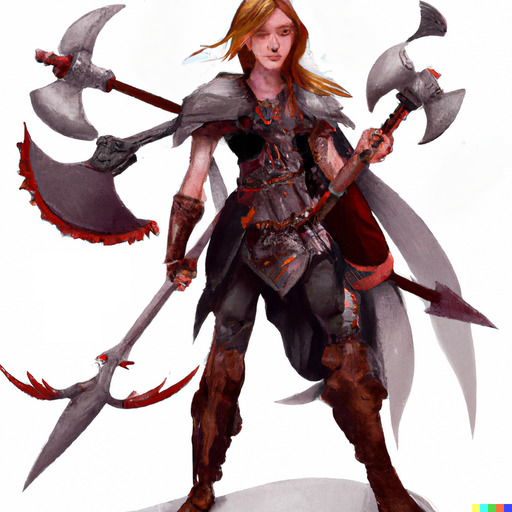
\includegraphics[width=\columnwidth]{equipment/weapons}

    Each weapon has a \glossterm{weapon group}, a \glossterm{usage class}, and any number of \glossterm{weapon tags}.
    In addition, each weapon has a particular \glossterm{accuracy} modifier and defines a base \glossterm{dice pool} for attacks using that weapon.
    This section explains each of those concepts and defines the statistics for weapons in Rise.
    You gain a \plus1d bonus to your \glossterm{weapon damage} per 2 power (see \pcref{Weapon Damage}).

    \subsection{Weapon Groups}\label{Weapon Groups}

        Weapons are organized into thematically related categories called weapon groups. They are described in \trefnp{Weapon Groups}. For example, all axes belong to the ``axes'' weapon group. Some weapons can be found in multiple weapon groups. For example, a dagger is a simple weapon, a blade, and a thrown weapon.

        \parhead{Exotic Weapons}\label{Exotic Weapons} Some weapons are rare and have unusual fighting styles.
        These weapons are called exotic weapons.
        Proficiency with a weapon group does not grant you with exotic weapons from that group.
        Some class abilities grant proficiency with exotic weapons.

        \begin{dtable!*}
            \lcaption{Weapon Groups}
            \begin{dtabularx}{\textwidth}{l >{\lcol}X >{\lcol}X}
                \tb{Group}         & \tb{Weapons}                                                                     & \tb{Exotic Weapons} \tableheaderrule
                Armor weapons      & Armor spikes, standard shield, spiked shield                                     & Armblade, spiked knee                                      \\
                Axes               & Battleaxe, broadaxe, greataxe, handaxe, poleaxe, shepherd's axe, throwing axe    & Dwarven throwing axe, dwarven waraxe, orcish greataxe      \\
                Blades             & Broadsword, dagger, estoc, greatsword, rapier, scimitar, smallsword              & Boot dagger, falchion, katana, kukri                       \\
                Bows               & Longbow, shortbow                                                                & Flatbow, heartseeker arrows, takedown bow                  \\
                Club-like weapons  & Club, flanged mace, greatmace, mace, morning star, sap                              & Culacula, gnomish trick mace, knobkerrie, totokia          \\
                Crossbows          & Hand crossbow, heavy crossbow                                                    & Arbalest, repeating crossbow                               \\
                Flexible Weapons   & Flail, heavy flail, nunchaku, slapjack, whip                                     & Chain whip, meteor hammer, three-section staff             \\
                Headed weapons     & Light hammer, longhammer, pick, sickle, sledgehammer, warhammer                  & Dwarven longhammer, dwarven shorthammer, heavy pick, obuch \\
                Improvised weapons & \tdash                                                                           & \tdash                                                     \\
                Monk weapons       & Jitte, kama, kunai, nunchaku, quarterstaff, sai, shuriken                        & Three-section staff                                        \\
                Polearms           & Bardiche, glaive, halberd, longhammer, poleaxe, quarterstaff, scythe, swordstaff & Fauchard, war scythe                                       \\
                Simple weapons     & Club, dagger, mace, quarterstaff                          & \tdash                                                     \\
                Spears             & Greatspear, javelin, lance, ranseur, partisan, spear                             & Gnomish smallspear, pike                                   \\
                Thrown weapons     & Dagger, dart, handaxe, javelin, light hammer, shuriken, sling, throwing axe      & Bolas, dwarven throwing axe, dwarven waraxe, net           \\
            \end{dtabularx}
        \end{dtable!*}

        \subsubsection{Weapon Proficiency}\label{Weapon Proficiency}
            Each character is proficient with different weapon groups. These indicate the weapons that you can use effectively.
            You take a \minus2 accuracy penalty with weapons you are not proficient with.

        \subsubsection{Improvised Weapons}\label{Improvised Weapons}
            Sometimes objects not crafted to be weapons nonetheless see use in combat.
            You can choose to be proficient with the improvised weapons weapon group, which has no specific weapons associated with it but which allows you to pick up and use non-manufactured weapons without taking a nonproficiency penalty (see \pcref{Weapon Proficiency}).

            To determine the appropriate statistics for an improvised weapon, compare its shape and composition to the weapon list to find a reasonable match.
            An improvised weapon will generally have a \minus1 accuracy penalty, a \minus1d damage penalty, or be missing at least one weapon tag relative to a similarly structured manufactured weapon.

        \subsubsection{Natural Weapons}\label{Natural Weapons}
            Natural weapons are weapons that are part of a creature's body instead of being manufactured and wielded.
            Many monsters have natural weapons, like claws or a bite attack.
            Natural weapons do not normally require a \glossterm{free hand} to use.
            All bipedal creatures also have a punch/kick natural weapon.

    \subsection{Weapon Usage Classes}\label{Weapon Usage Classes}
        A weapon's \glossterm{usage class} is a measure of how much effort it takes to wield a weapon in combat.
        It indicates whether a weapon, when wielded by a creature the weapon is sized for, is considered a light weapon, a medium weapon, or a heavy weapon.

        % All weapons should have two improvements over a ``baseline'' +0/+0d weapon with no properties.
        % In addition, light and heavy weapons have additional properties that are not considered improvements.
        % Being Light grants an automatic +1a/-1d and better dual wielding/grappling, and light weapons cannot be higher than 1d6 base.
        % Being Medium has no special properties, but many Medium weapons have the Versatile Grip property.
        % Being Heavy grants an automatic +1d, but all heavy weapons require two hands.
        % Extreme weapons are discouraged; although this permits a 2d8 Heavy weapon, no such weapon should exist.
        % Trading -1d/+1a or +1d/-1a is not considered an improvement.

        % Accuracy/damage math:
        % Assume 60% hit chance and 1d10+4 damage as a typical value. That's 9.5dph, or 5.7dpr.
        % +1d (2d6) is about 25% more damage from dice. That's 11 dph (16% more) and 6.6 dpr (16% more)
        % +2d (2d8) is about 60% more damage from dice. That's 13 dph (37% more) and 7.8 dpr (37% more)
        % +1a is 6.6 dpr (16% more), and +2a is 7.6 dpr (33% more)

        % Crit math:
        % 10% chance to explode, 60% chance to hit on explosion, so 6% chance to crit.
        % Base damage per crit (dpc) is 5.5, so 0.33 dpr from crits, or 6.03 damage per round with crits (dprc).
        % On sneak attack / smite / similar abilities, 9.5dpc, so 0.57 dpr from crits, or 6.27 dprc
        % Keen (+2): +2% chance to crit, +0.11 dpr, 6.14 dprc (1% more)
        % Keen sneak attack: +2% chance to crit, +0.19 dpr, 6.22 dprc (3% more)
        % Impact: +5.5 dpc, +0.33 dpr, 6.36 dprc (5% more)
        % Impact sneak attack: +9.5 dpc, +0.57 dpr, 6.6 dprc (9% more)
        % Summary: Crit abilities are *catastrophically terrible*.
        % But that doesn't tell the whole story, because you're often crit-fishing.

        % Desperate exertion crit math:
        % output [highest of [explode 1d10] and [explode 1d10]] >= 15
        % 11.6% crit chance, 0.64 dpr from crits, 6.34 dprc
        % Sneak attack: 9.5 dpc, 1.1 dpr from crits, 7.13 dprc
        % Keen: 15.4% crit chance, 0.85 dpr from crits, 6.55 dprc (3% more)
        % Impact: +5.5 dpc, +0.64 dpr from crits, 6.67 dprc (10% more)
        % Impact sneak attack: +9.5 dpc, +1.1 dpr from crits, 8.23 dprc (15% more)
        % Summary: Keen is still terrible.
        % Impact is more compelling, and scales well if you can get crit chance higher (totem barbarian)

        % Heavy weapon math:
        % Assume a duel between a 2d6+4 greataxe (40% hit chance) and a 1d8+4 shield user (60% hit chance)
        % Greataxe is 4.4 dpr, shield is 5.7 dpr
        % Using a shield is still clearly superior in a duel context, even with +2d on heavy weapons.

        % This means the template, unimproved weapons are:
        % Light: +1a, 1d4 damage
        % Medium: +0a, 1d6 damage
        % Heavy: +0a, 1d10 damage

        \parhead{Light Weapons}\label{Light Weapons} Light weapons are easier to use while making attacking with two weapons at once (see \pcref{Offhand Strike}) or while grappling.
        They cannot be held in two hands.
        Light weapons tend to have higher \glossterm{accuracy} than heavier weapons, but do less damage.

        \parhead{Medium Weapon} A medium weapon can normally be used in one hand.
        Most medium weapons can also be held in two hands if that is physically plausible.
        This provides no special benefit unless the weapon has the Versatile Grip tag (see \pcref{Weapon Tags}).
        Changing grips to hold it in one hand or two hands can be done as a \glossterm{free action} that requires both hands.

        \parhead{Heavy Weapon} Two hands are normally required to wield a heavy weapon.
        Heavy weapons tend to have higher damage than lighter weapons.
        If you have a Strength of 3 or higher, you can wield a heavy weapon in one hand, but you take a \minus1 penalty to \glossterm{accuracy} and a \minus1d damage penalty with the weapon while doing so.
        You can change your grip on a heavy weapon as a \glossterm{free action}.

        \parhead{Physical Size} Like all objects and creatures, weapons have a size category that represents how physically large they are. In general, light and medium weapons are one size category smaller than the wielder, while heavy weapons are the same size category as the wielder.
        All weapons are \glossterm{lightweight} unless otherwise noted.

        \parhead{Inappropriately Sized Weapons}\label{Inappropriately Sized Weapons} A weapon's \glossterm{usage class} is altered by one step for each size category of difference between the wielder's size and the size of the creature for which the weapon was designed.
        For example, a light weapon sized for a Large creature can be used by a Medium creature as if it had a medium usage class.
        The weapon's damage die gains a \plus1d bonus per size category if the weapon is unusually large, or takes a \minus1d penalty per size category if the weapon is unusually small.
        In addition, the wielder takes a \minus2 accuracy penalty with the weapon per size category of difference.
        If a weapon's usage class would be changed to something other than light, medium, or heavy by this alteration, the creature can't wield the weapon at all.

    \subsection{Weapon Range Limits}\label{Weapon Range Limits}
        Ranged weapon attacks become less accurate if the target is far away.
        Ranged weapons have two \glossterm{range limits} listed, with a slash between them, such as 90/270.
        The first number indicates the maximum range for a weapon's \glossterm{close range}.
        The second number indicates the maximum range for a weapon's \glossterm{long range}.
        You cannot attack a target that is beyond a weapon's long range limit.

        Attacks at close range have no penalty.
        Attacks at long range have a \minus4 accuracy penalty.
        This is called a \glossterm{longshot penalty}, and some abilities can reduce this penalty.

    \subsection{Drawing and Sheathing Weapons}\label{Drawing and Sheathing Weapons}
        Drawing and sheathing weapons always requires the hand or hands used to hold the weapon.
        The time it takes to draw and sheathe a weapon depends on how encumbering the weapon is.
        As a \glossterm{free action}, you can draw or sheathe a single \glossterm{medium weapon} or up to two \glossterm{light weapons}, assuming they are easy to access.
        Like other free actions, you cannot take this action twice in the same round, so you cannot draw and sheathe weapons in the same round.
        As a standard action, you can draw or sheathe any of the following equipment combinations: up to two \glossterm{medium weapons}, a medium weapon and a shield, one \glossterm{heavy weapon}, or one weapon that is concealed or otherwise difficult to access.

        A character can only store a limited number of weapons in locations that are easy to access in combat.
        Generally, a humanoid creature is limited to four light weapons, two shields or non-heavy weapons, and one weapon of any usage class.
        For each weapon or shield stored in easily accessible locations in excess of this limit, the character increases their \glossterm{encumbrance} by 1.

    \subsection{Weapon Tags}\label{Weapon Tags}
        Some weapons found on \trefnp{Weapons} have tags that indicate that they have special abilities. The list of abilities that weapons can have is given below.
        \weapontagdef{Supplemental} This weapon has some unusual purpose, rather than exclusively functioning as a weapon.
        Supplemental weapons cannot be imbued with magic weapon properties.
        Most Supplemental weapons are part of armor.
        \weapontagdef{Ammunition} This weapon is designed to be fired by a projectile weapon or thrown in large quantities.
        It is cheaper to buy and craft, but it is usually \glossterm{broken} after being fired or thrown.
        \weapontagdef{Compact} This weapon is unusually small.
        It is one size category smaller than normal for a light weapon (that is, two size categories smaller than the creature it is intended for), though it is not \glossterm{lightweight} for that size.
        This makes it easier to conceal (see \pcref{Sleight of Hand}).
        In addition, you can draw or sheathe this weapon so quickly that you can also take another action in the same phase with that hand.
        For example, you can draw this weapon and attack with it in the same phase.
        \weapontagdef{Forceful} Whenever you deal damage to a target no more than one size category larger than you with a strike using this weapon, you can \glossterm{knockback} the target up to 10 feet.
        On a critical hit, this knockback distance is doubled.
        \weapontagdef{Grappling} You gain a \plus2 bonus to \glossterm{accuracy} on \glossterm{melee} attacks with this weapon against creatures who are \grappled by you.
        \weapontagdef{Impact} When you get a \glossterm{critical hit} with this weapon, you roll triple damage dice instead of double damage dice.
        \weapontagdef{Keen} You gain a \plus4 bonus to \glossterm{accuracy} with \glossterm{strikes} using this weapon for the purpose of determining whether you get a \glossterm{critical hit}.
        \weapontagdef{Long}\label{Long Weapon} This weapon can be used to make melee \glossterm{strikes} against targets up to 10 feet away from you.
        If you use an ability with more specific targets than simply making a melee strike, such as affecting ``all enemies adjacent to you'', this weapon tag does not increase your range with that ability.
        In addition, you can inflict \glossterm{critical hits} with melee \glossterm{strikes} using a Long weapon against creatures up to two size categories larger than you (see \pcref{Very Large Creatures}).
        \weapontagdef{Mounted}\label{Mounted Weapon} If you are mounted, and your mount moves in the same phase that you make a \glossterm{strike} with a Mounted weapon, you gain a \plus2 \glossterm{accuracy} bonus with the strike.
        \weapontagdef{Parrying} If a creature attacks you with a \glossterm{melee} \glossterm{strike} while you wield this weapon, you \glossterm{briefly} gain a \plus2 bonus to \glossterm{accuracy} with strikes using this weapon against that creature.
        \weapontagdef{Projectile} This weapon fires ammunition at range to deal damage.
        The ammunition generally breaks when used.
        Projectile weapons have two \glossterm{range limits} listed in their description (see \pcref{Weapon Range Limits}).
        They must be reloaded after being fired.
        The time required to reload a projectile weapon is given in the weapon description.
        You take a \minus4 accuracy penalty with Projectile weapons against creatures adjacent to you.
        While mounted, you take a \minus4 accuracy penalty with Projectile weapons, and your range limits are halved.
        \weapontagdef{Stealthy}
        A stealthy weapon is smaller, quieter, or otherwise less noticeable than most weapons.
        You only take a \minus5 penalty to Stealth when trying to conceal strikes with a stealthy weapon instead of the normal \minus10 or \minus20 penalty for concealing a strike (see \pcref{Stealth}).
        \weapontagdef{Sweeping}\label{Sweeping} When you make a \glossterm{melee} \glossterm{strike} with this weapon, you may also target one or more secondary creatures or objects adjacent to you.
        If the weapon also has the \weapontag{Long} weapon tag, each secondary target may instead be within 10 feet of you.
        Each secondary target must be within 10 feet of a primary target, and must not already be a target of the strike.
        The strike affects each secondary target in the same way as the primary targets.
        Sweeping weapons have a number that indicates the number of secondary targets you can affect.
        \weapontagdef{Subdual} This weapon deals \glossterm{subdual damage} (see \pcref{Subdual Damage}).
        % (30/60) is one improvement, (60/120) is two.
        \weapontagdef{Thrown} This weapon is designed to be thrown to deal damage at range.
        Thrown weapons have two \glossterm{range limits} listed in their description (see \pcref{Weapon Range Limits}).
        Unless otherwise noted in a weapon's description, a throwing weapon can be used to attack in melee without penalty.

        Heavy thrown weapons require a standard action to throw, rather being thrown as part of any \glossterm{strike} like normal.
        They are not always physically thrown with two hands, but they require the use of your entire body to propel the weapon, so you are not considered to have any \glossterm{free hands} while throwing a heavy thrown weapon.
        \weapontagdef{Tripping} When you use the \ability{trip} ability, you can attack with this weapon instead of with a free hand (see \pcref{Trip}).
        This allows you to deal damage with the weapon if you successfully trip the target.
        \weapontagdef{Versatile Grip} This weapon is designed to be held in either one hand or two hands.
        While holding this weapon in two hands, you gain a \plus2d damage bonus with it.

    \subsection{Weapon Table}
        Here is the format for weapon entries in the Weapons table, below.

        \parhead{Usage Class} Describes whether the weapon's \glossterm{usage class} is light, medium, or heavy (see \pcref{Weapon Usage Classes}).

        \parhead{Accuracy} This number modifies your \glossterm{accuracy} with \glossterm{strikes} using the weapon.

        \parhead{Damage} This \glossterm{dice pool} indicates the damage dealt by the weapon on a hit.

        \parhead{Damage Type} This indicates the type of the damage dealt by the weapon.
        Some monsters may be \trait{impervious} or immune to attacks from certain damage types.

        Some weapons deal damage of multiple types. If a weapon is of two types, the damage it deals is not half one type and half another; all of it is both types.
        Therefore, a creature would have to be immune to both types of damage to ignore any of the damage from such a weapon.
        For details, see \pcref{Multiple Damage Types}.

        In other cases, a weapon can deal either of two types of damage.
        The wielder chooses which type of damage to deal when they make each \glossterm{strike} with the weapon.

        \parhead{Item Rank (Cost)} The first value indicates the \glossterm{item rank} of the item (see \pcref{Item Ranks}).
        The second value in parentheses indicates the average cost to buy the item.
        Items crafted for unusually large or small creatures are more expensive.
        For each size category larger or smaller than Medium, the item's rank increases by one, which increases its price.

        \parhead{Weapon Tags} Some weapons have special properties. See \pcref{Weapon Tags} for details.

        \begin{longtablewrapper}
            \tablebookmark{Weapons}{weapons}
            \RaggedRight
            \begin{longtable}{p{10em} c c c >{\ccol}p{7em} c >{\ccol}p{12em}}
                \lcaption{Weapons}                     \\
                \tb{Name}                          & \tb{Usage Class} & \tb{Accuracy} & \tb{Damage} & \tb{Damage Type}   & \tb{Item Rank (Cost)}\fn{1} & \tb{Weapon Tags}                          \tableheaderrule
                Armor weapons                      &        &         &        &                          &           &                                                \\
                \tind Armor spikes\fn{2}           & Medium & \tdash  & 1d4    & Piercing                 & \tdash    & Supplemental                                   \\
                \tind Standard shield\fn{3}        & Medium & \plus0  & 1d4    & Bludgeoning              & 0 (10 gp) & Supplemental                                   \\
                \tind Spiked standard shield\fn{3} & Medium & \plus0  & 1d6    & Bludgeoning and piercing & 1 (40 gp) & Supplemental                                   \\

                Axes                               &        &         &        &                          &           &                                                \\
                \tind Battleaxe                    & Medium & \plus0  & 1d8    & Slashing                 & 0 (10 gp) & Versatile Grip                   \\
                \tind Broadaxe                     & Medium & \plus0  & 1d6    & Slashing                 & 0 (10 gp) & Sweeping (1), Versatile Grip                   \\
                \tind Greataxe                     & Heavy  & \plus0  & 2d6    & Slashing                 & 0 (10 gp) & Sweeping (1)                                   \\
                \tind Handaxe                      & Light  & \plus1  & 1d6    & Slashing                 & 0 (10 gp) & Thrown (30/60)                                 \\
                \tind Poleaxe                      & Heavy  & \plus0  & 1d10    & Piercing or slashing     & 0 (10 gp) & Impact, Tripping                               \\
                \tind Shepherd's axe               & Light  & \plus1  & 1d6    & Bludgeoning or slashing  & 0 (10 gp) & Long                                           \\
                \tind Throwing axe                 & Medium & \plus0  & 1d8    & Slashing                 & 0 (10 gp) & Thrown (30/60)                         \\

                Blades                             &        &         &        &                          &           &                                                \\
                \tind Broadsword                   & Medium & \plus0  & 1d6    & Slashing                 & 0 (10 gp) & Sweeping (1), Versatile Grip                   \\
                \tind Dagger                       & Light  & \plus2  & 1d3    & Piercing or slashing     & 0 (10 gp) & Compact, Thrown (30/60), Stealthy              \\
                \tind Estoc                        & Medium & \plus0  & 1d6    & Piercing                 & 0 (10 gp) & Long, Versatile Grip                           \\
                \tind Greatsword                   & Heavy  & \plus0  & 1d10    & Slashing                 & 0 (10 gp) & Sweeping (2)                                   \\
                \tind Rapier                       & Light  & \plus2  & 1d6    & Piercing                 & 0 (10 gp) & \tdash                                           \\
                \tind Scimitar                     & Medium & \plus0  & 1d6    & Slashing                 & 0 (10 gp) & Keen, Mounted                                  \\
                \tind Smallsword                   & Light  & \plus2  & 1d4    & Piercing                 & 0 (10 gp) & Keen                                           \\

                Bows                               &        &         &        &                          &           &                                                \\
                \tind Longbow\fn{2}                & Heavy  & \plus0  & 1d6    & \tdash                   & 1 (40 gp) & Projectile (90/270)                            \\
                \tind Shortbow\fn{2}               & Medium & \plus0  & 1d4    & \tdash                   & 1 (40 gp) & Projectile (60/180), Stealthy                  \\
                \tind Arrows (20)                  & \tdash & \plus0  & \tdash & Piercing                 & 0 (2 gp)  & Ammunition                                     \\
                \tind Blunted arrows (20)          & \tdash & \minus1 & \tdash & Bludgeoning              & 0 (2 gp)  & Ammunition, Subdual                            \\
                \tind Fire arrows (20)\fn{2}       & \tdash & \minus1 & \tdash & Piercing and fire        & 2 (25 gp) & Ammunition                                     \\

                Club-like weapons                  &        &         &        &                          &           &                                                \\
                \tind Cavalry mace                 & Medium & \plus0  & 1d6    & Bludgeoning              & 0 (10 gp) & Mounted, Versatile Grip                                 \\
                % only 1 improvement
                \tind Club                         & Medium & \plus0  & 1d8   & Bludgeoning              & 0         & \tdash                                         \\
                \tind Flanged mace                 & Medium & \plus0  & 1d6    & Bludgeoning              & 0 (10 gp) & Impact                         \\
                \tind Greatmace                    & Heavy  & \plus0  & 2d6   & Bludgeoning              & 0 (10 gp) & Impact                                         \\
                % only 1 improvement
                \tind Mace                         & Medium & \plus0  & 1d6    & Bludgeoning              & 0 (10 gp) & Impact                         \\
                \tind Morning star                 & Medium & \plus0  & 1d8    & Bludgeoning and piercing & 0 (10 gp) & Versatile Grip                                 \\
                \tind Sap                          & Light  & \plus2  & 1d3    & Bludgeoning              & 0 (10 gp) & Stealthy, Subdual                              \\

                Crossbows                          &        &         &        &                          &           &                                                \\
                \tind Hand crossbow\fn{2}          & Light  & \plus1  & 1d3    & \tdash                   & 1 (40 gp) & Projectile (30/90), Stealthy                   \\
                \tind Heavy crossbow\fn{2}         & Heavy  & \plus0  & 1d10   & \tdash                   & 1 (40 gp) & Projectile (90/270)                            \\
                \tind Crossbow bolts (20)          & \tdash & \plus0  & \tdash & Piercing                 & 0 (2 gp)  & Ammunition                                     \\
                \tind Blunted crossbow bolts (20)  & \tdash & \minus1 & \tdash & Piercing                 & 0 (2 gp)  & Ammunition, Subdual                            \\

                Flexible weapons                   &        &         &        &                          &           &                                                \\
                \tind Flail                        & Medium & \plus0  & 1d6    & Bludgeoning              & 0 (10 gp) & Tripping, Versatile Grip                       \\
                \tind Heavy flail                  & Heavy  & \plus0  & 2d6   & Bludgeoning              & 0 (10 gp) & Tripping                                       \\
                \tind Two-section staff            & Heavy  & \plus1  & 1d8    & Bludgeoning              & 0 (10 gp) & Long, Tripping                                 \\
                \tind Nunchaku                     & Light  & \plus2  & 1d4    & Bludgeoning              & 0 (10 gp) & Tripping                                       \\
                \tind Slapjack                     & Light  & \plus2  & 1d4    & Bludgeoning              & 0 (10 gp) & Subdual                                        \\
                \tind Whip\fn{2}                   & Medium & \plus0  & 1d4    & Bludgeoning              & 0 (10 gp) & Long, Subdual, Tripping                        \\

                Headed weapons                     &        &         &        &                          &           &                                                \\
                \tind Light hammer                 & Light  & \plus1  & 1d6    & Bludgeoning              & 0 (10 gp) & Thrown (30/60)                       \\
                \tind Longhammer                   & Heavy  & \plus0  & 1d10    & Bludgeoning              & 0 (10 gp) & Forceful, Long                                 \\
                \tind Pick                         & Medium & \plus0  & 1d6    & Piercing                 & 0 (10 gp) & Impact, Versatile Grip                         \\
                \tind Sickle                       & Light  & \plus1  & 1d4    & Slashing                 & 0 (10 gp) & Sweeping (1), Tripping                                       \\
                \tind Sledgehammer                 & Heavy  & \plus0  & 2d6   & Bludgeoning              & 0 (10 gp) & Forceful                                       \\
                \tind Warhammer                    & Medium & \plus0  & 1d6    & Bludgeoning              & 0 (10 gp) & Forceful, Versatile Grip                       \\

                Monk weapons                       &        &         &        &                          &           &                                                \\
                \tind Jitte                        & Light  & \plus2  & 1d4    & Piercing                 & 0 (10 gp) & Parrying                                       \\
                \tind Kama                         & Light  & \plus2  & 1d4    & Slashing                 & 0 (10 gp) & Tripping                                       \\
                \tind Kunai                        & Light  & \plus1  & 1d4    & Piercing                 & 0 (10 gp) & Thrown (60/120)                                \\
                \tind Nunchaku                     & Light  & \plus2  & 1d4    & Bludgeoning              & 0 (10 gp) & Tripping                                       \\
                % Only one improvement
                \tind Quarterstaff                 & Heavy  & \plus1  & 1d8   & Bludgeoning              & 0         & Long                                           \\
                \tind Shuriken (5)                 & Light  & \plus2  & 1d3    & Piercing and slashing    & 0 (10 gp) & Ammunition, Compact, Thrown (30/60), Stealthy  \\

                Polearms                           &        &         &        &                          &           &                                                \\
                \tind Bardiche                     & Heavy  & \plus0  & 2d6   & Slashing                 & 0 (10 gp) & Sweeping (1)                                   \\
                \tind Glaive                       & Heavy  & \plus0  & 1d10    & Slashing                 & 0 (10 gp) & Long, Sweeping (1)                             \\
                \tind Halberd                      & Heavy  & \plus0  & 1d10    & Piercing or slashing     & 0 (10 gp) & Long, Tripping                                 \\
                \tind Longhammer                   & Heavy  & \plus0  & 1d10    & Bludgeoning              & 0 (10 gp) & Forceful, Long                                 \\
                \tind Poleaxe                      & Heavy  & \plus0  & 1d10    & Piercing or slashing     & 0 (10 gp) & Impact, Tripping                               \\
                % Only one improvement
                \tind Quarterstaff                 & Heavy  & \plus1  & 1d8   & Bludgeoning              & 0         & Long                                           \\
                \tind Scythe                       & Heavy  & \plus0  & 1d10    & Slashing                 & 0 (10 gp) & Sweeping (2)                                   \\
                \tind Swordstaff                   & Heavy  & \plus1  & 1d10    & Slashing                 & 0 (10 gp) & Long                                     \\

                Simple weapons                     &        &         &        &                          &           &                                                \\
                \tind Claw sheathe\fn{2}           & \tdash & \tdash  & \tdash & \tdash                   & 1 (40 gp) & \tdash                                         \\
                % only 1 improvement
                \tind Club                         & Medium & \plus0  & 1d8   & Bludgeoning              & 0         & \tdash                                         \\
                \tind Dagger                       & Light  & \plus2  & 1d3    & Piercing or slashing     & 0 (10 gp) & Compact, Stealthy, Thrown (30/60)              \\
                % only 1 improvement
                \tind Mace                         & Medium & \plus0  & 1d6    & Bludgeoning              & 0 (10 gp) & Impact                         \\
                % only 1 improvement
                \tind Quarterstaff                 & Heavy  & \plus1  & 1d8    & Bludgeoning              & 0         & Long                                           \\

                Spears                             &        &         &        &                          &           &                                                \\
                \tind Greatspear                   & Heavy  & \plus0  & 2d6   & Piercing                 & 0 (10 gp) & Long                                           \\
                \tind Javelin                      & Medium & \plus0  & 1d6    & Piercing                 & 0 (10 gp) & Thrown (60/120)                                \\
                \tind Lance                        & Heavy  & \plus0  & 1d10    & Piercing                 & 0 (10 gp) & Long, Mounted                                  \\
                \tind Ranseur                      & Heavy  & \plus2  & 1d8    & Piercing                 & 0 (10 gp) & Long                                           \\
                \tind Spear                        & Medium & \plus0  & 1d6    & Piercing                 & 0 (10 gp) & Thrown (30/60), Versatile Grip                 \\

                Thrown weapons                     &        &         &        &                          &           &                                                \\
                \tind Dagger                       & Light  & \plus2  & 1d3    & Piercing or slashing     & 0 (10 gp) & Compact, Stealthy, Thrown (30/60)              \\
                \tind Dart (5)                     & Light  & \plus1  & 1d3    & Piercing                 & 0 (2 gp)  & Ammunition, Compact, Thrown (60/120), Stealthy \\
                \tind Handaxe                      & Light  & \plus1  & 1d6    & Slashing                 & 0 (10 gp) & Thrown (30/60)                                 \\
                \tind Light hammer                 & Light  & \plus1  & 1d6    & Bludgeoning              & 0 (10 gp) & Thrown (30/60)                       \\
                \tind Javelin                      & Medium & \plus0  & 1d6    & Piercing                 & 0 (10 gp) & Thrown (60/120)                                \\
                \tind Shuriken (5)                 & Light  & \plus2  & 1d3    & Piercing and slashing    & 0 (2 gp)  & Ammunition, Compact, Thrown (30/60), Stealthy  \\
                \tind Sling\fn{2}                  & Light  & \plus0  & 1d4    & Bludgeoning              & 0 (10 gp) & Projectile (90/270)                            \\
                \tind Throwing axe                 & Medium & \plus0  & 1d8    & Slashing                 & 0 (10 gp) & Thrown (30/60)                         \\
                \tind Bullets, sling (20)          & \tdash & \tdash  & \tdash & \tdash                   & 0 (2 gp)  & Ammunition                                     \\

                % Exotic weapons should be +3 over normal
                \tb{Exotic Weapons}\label{Exotic Weapons} & \tb{Usage Class} & \tb{Accuracy} & \tb{Damage} & \tb{Damage Type} & \tb{Item Rank (Cost)}\fn{1} & \tb{Weapon Tags} \tableheaderrule
                Armor                           &         &        &         &                          &            &                                    \\
                \tind Armblade\fn{2}            & Light   & \plus2 & 1d4     & Slashing                 & 1 (40 gp)  & Grappling, Keen, Supplemental      \\
                \tind Spiked knee\fn{2}         & Light   & \plus1 & 1d4     & Piercing                 & 1 (40 gp)  & Grappling, Impact, Supplemental    \\
                \tind Tower shield\fn{3}        & Heavy   & \plus0 & 1d10    & Bludgeoning              & 1 (40 gp)  & Supplemental                       \\
                \tind Spiked tower shield\fn{3} & Heavy   & \plus0 & 2d6    & Bludgeoning and piercing & 1 (40 gp)  & Supplemental                       \\
                Axes                            &         &        &         &                          &            &                                    \\
                \tind Dwarven throwing axe      & Medium  & \plus0 & 1d8     & Slashing                 & 0 (10 gp)  & Thrown (60/120)            \\
                \tind Dwarven waraxe            & Medium  & \plus0 & 1d8     & Slashing                 & 1 (40 gp)  & Thrown (30/60), Versatile Grip     \\
                \tind Orcish greataxe           & Heavy   & \plus0 & 2d6    & Slashing                 & 1 (40 gp)  & Impact, Sweeping (1)               \\
                Blades                          &         &        &         &                          &            &                                    \\
                \tind Boot dagger\fn{2}         & Light   & \plus2 & 1d4     & Piercing                 & 0 (10 gp)  & Compact, Stealthy, Supplemental    \\
                \tind Falchion                  & Medium  & \plus0 & 1d6     & Slashing                 & 1 (40 gp)  & Sweeping (2), Versatile Grip       \\
                \tind Katana                    & Heavy   & \plus2 & 1d8     & Slashing                 & 1 (40 gp)  & Keen, Sweeping (1)                 \\
                \tind Kukri                     & Light   & \plus2 & 1d4     & Slashing                 & 0 (10 gp)  & Keen, Sweeping (1)                 \\
                \tind Parrying dagger           & Light   & \plus2 & 1d4     & Piercing                 & 0 (10 gp)  & Parrying, Stealthy, Thrown (30/60) \\
                Bows                            &         &        &         &                          &            &                                    \\
                \tind Flatbow\fn{2}             & Heavy   & \plus1 & 1d6     & \tdash                   & 1 (40 gp)  & Projectile (90/270)                \\
                \tind Heartseeker arrows (20)   & \tdash  & \plus0 & \tdash  & Piercing                 & 2 (40 gp)  & Ammunition, Impact                 \\
                \tind Takedown bow\fn{2}        & Special & \plus0 & 1d6/1d4 & \tdash                   & 2 (200 gp) & Projectile (90/270 or 60/180)      \\
                Club-like weapons               &         &        &         &                          &            &                                    \\
                \tind Culacula                  & Heavy   & \plus0 & 1d10    & Bludgeoning              & 0 (10 gp)  & Forceful, Impact, Parrying         \\
                \tind Gnomish trick mace        & Light   & \plus2 & 1d4     & Bludgeoning              & 0 (10 gp)  & Impact, Tripping                   \\
                \tind Knobkerrie                & Medium  & \plus1 & 1d6     & Bludgeoning              & 0 (10 gp)  & Impact, Throwing (30/60)           \\
                \tind Totokia                   & Medium  & \plus0 & 1d8     & Bludgeoning and piercing & 0 (10 gp)  & Impact, Versatile Grip             \\
                Crossbows                       &         &        &         &                          &            &                                    \\
                \tind Arbalest\fn{2}            & Heavy   & \plus2 & 1d10    & \tdash                   & 2 (200 gp) & Impact, Projectile (90/270)        \\
                \tind Repeating crossbow\fn{2}  & Medium  & \plus0 & 1d6     & \tdash                   & 2 (200 gp) & Impact, Projectile (90/270)        \\
                \tind Repeating bolts (5)       & \tdash  & \plus0 & \tdash  & Piercing                 & 1 (10 gp)  & Ammunition                         \\
                Flexible weapons                &         &        &         &                          &            &                                    \\
                \tind Bladed whip\fn{2}         & Medium  & \plus0 & 1d6     & Slashing                 & 1 (40 gp)  & Keen, Long, Sweeping (1)                 \\
                \tind Chain whip                & Medium  & \plus0 & 1d8     & Bludgeoning              & 1 (40 gp)  & Long, Tripping                     \\
                \tind Meteor hammer             & Heavy   & \plus0 & 2d6    & Bludgeoning              & 1 (40 gp)  & Long, Tripping                     \\
                \tind Three-section staff       & Heavy   & \plus1 & 1d8     & Bludgeoning              & 1 (40 gp)  & Long, Parrying, Tripping           \\
                Headed weapons                  &         &        &         &                          &            &                                    \\
                \tind Dwarven longhammer        & Heavy   & \plus0 & 2d6    & Bludgeoning              & 1 (40 gp)  & Forceful, Long                     \\
                \tind Dwarven shorthammer       & Light   & \plus2 & 1d6     & Bludgeoning              & 1 (40 gp)  & Impact                   \\
                \tind Heavy pick                & Heavy   & \plus0 & 2d6     & Piercing                 & 1 (40 gp)  & Keen, Impact                       \\
                \tind Obuch                     & Medium  & \plus0 & 1d8     & Bludgeoning              & 1 (40 gp)  & Long, Tripping                     \\
                Monk weapons                    &         &        &         &                          &            &                                    \\
                \tind Sai                       & Light   & \plus2 & 1d4     & Piercing or bludgeoning  & 0 (10 gp)  & Grappling, Parrying                \\
                \tind Three-section staff       & Heavy   & \plus1 & 1d8     & Bludgeoning              & 1 (40 gp)  & Long, Parrying, Tripping           \\
                Polearms                        &         &        &         &                          &            &                                    \\
                \tind Fauchard                  & Heavy   & \plus0 & 1d10     & Slashing                 & 1 (40 gp)  & Long, Sweeping (2)                 \\
                \tind War scythe                & Heavy   & \plus1 & 1d10    & Slashing or piercing     & 1 (40 gp)  & Sweeping (2)                       \\
                Simple weapons                  &         &        &         &                          &            &                                    \\
                Spear                           &         &        &         &                          &            &                                    \\
                \tind Gnomish smallspear        & Light   & \plus2 & 1d6     & Piercing                 & 0 (10 gp)  & Long                       \\
                \tind Partisan                  & Heavy   & \plus1 & 1d10    & Piercing                 & 1 (40 gp)  & Parrying, Long                     \\
                \tind Pike\fn{2}                & Heavy   & \plus0 & 2d6    & Piercing                 & 0 (10 gp)  & Long                               \\
                Thrown weapons                  &         &        &         &                          &            &                                    \\
                % only two because thrown + tripping is extra good?
                \tind Bolas                     & Light   & \plus1 & 1d3     & Bludgeoning              & 0 (10 gp)  & Thrown (30/60), Tripping           \\
                \tind Dwarven throwing axe      & Medium  & \plus0 & 1d8     & Slashing                 & 0 (10 gp)  & Thrown (60/120)            \\
                \tind Dwarven waraxe            & Medium  & \plus0 & 1d8     & Slashing                 & 1 (40 gp)  & Thrown (30/60), Versatile Grip     \\
                \tind Net\fn{2}                 & Medium  & \plus0 & \tdash  & \tdash                   & 0 (10 gp)  & Supplemental, Thrown (5/15)        \\
            \end{longtable}
            1 See \pcref{Item Ranks}. \\
            2 This weapon has special rules. \\
            3 You cannot use the \ability{offhand strike} ability with a shield. \\
        \end{longtablewrapper}

        \begin{dtable!*}
            % Every natural weapon that requires a free hand should be on par with a manufactured weapon.
            % Every natural weapon that can be used with both hands occupied should be one upgrade behind an equivalent manufactured weapon.
            \tablebookmark{Natural Weapons}{naturalweapons}
            \lcaption{Natural Weapons}
            \begin{dtabularx}{\textwidth}{p{12em} c c c >{\ccol}p{15em} >{\ccol}X}
                \tb{Natural Weapons}    & \tb{Usage Class} & \tb{Accuracy} & \tb{Damage} & \tb{Damage Type} & \tb{Weapon Tags} \tableheaderrule
                Bite                    & Medium           & \plus0        & 1d6         & Physical         & Grappling      \\
                Claw\fn{1}              & Light            & \plus2        & 1d4         & Slashing         & Versatile Grip \\
                Gore                    & Medium           & \plus0        & 1d6         & Piercing         & Impact         \\
                Punch/kick\fn{1} \fn{2} & Light            & \plus0        & 1d3         & Bludgeoning      & Subdual        \\
                Ram                     & Medium           & \plus0        & 1d6         & Bludgeoning      & Forceful       \\
                Slam\fn{1}              & Medium           & \plus0        & 1d10        & Bludgeoning      & \tdash         \\
                Stinger                 & Medium           & \plus1        & 1d6         & Piercing         & \tdash         \\
                Talon\fn{1}             & Light            & \plus2        & 1d4         & Piercing         & Versatile Grip \\
            \end{dtabularx}
            1 This natural weapon must normally be used with a \glossterm{free hand}. \\
            2 This weapon has special rules. \\
        \end{dtable!*}

    \subsection{Individual Weapon Descriptions}
        Some weapons in \trefnp{Weapons} have additional abilities which are described below.
        \parhead{Arbalest} You draw an arbalest back by turning a small winch. Loading an arbalest requires two standard actions.
        Each standard action requires one \glossterm{free hand} while holding the arbalest in another hand.
        \parhead{Armblade} This weapon is not held in a hand.
        Instead, it is affixed to the arm of body armor with a medium or heavy \glossterm{usage class}.
        When you attack with an armblade, you cannot use the arm it is attached to for any other combat purpose in the same phase.
        You can still hold items in that hand, but they have no combat effect.
        If you are not proficient with this weapon, you increase your \glossterm{encumbrance} by 2 when wearing armor with an armblade.
        \parhead{Armor Spikes} Any \glossterm{body armor} can be spiked.
        You cannot normally attack with armor spikes.
        However, if your armor is spiked and you are proficient with it, you deal damage with it when you make a successful \textit{grapple} or \textit{shove} attack.
        Your \glossterm{power} is halved for the purpose of this damage, and this damage is not doubled if you get a critical hit with the grapple or shove attack.
        This damage cannot be combined with other effects that deal damage with a shove.
        \parhead{Bladed Whip} A bladed whip can be used to attack targets within 15 feet instead of the normal 10 feet for a Long weapon.
        \parhead{Boot Dagger} A boot dagger is a modified boot or boot sole which contains a hidden dagger.
        The dagger is normally concealed, and requires an Awareness check with a \glossterm{difficulty value} of 15 to find.
        Attacking with a boot dagger does not require a \glossterm{free hand}, but you must make a Balance check with a \glossterm{difficulty value} of 10 during whenever you attack with it.
        If you fail this check, you fall \prone after the attack.

        After you attack with a boot dagger, the dagger remains plainly visible.
        Concealing the dagger again requires a standard action.
        \parhead{Claw} This weapon has the Versatile Grip tag, which may seem odd for an obviously one-handed weapon.
        The damage bonus from that tag represents attacking with claws on both hands at once, rather than grabbing one claw with both hands.
        If a creature only has a claw on a single hand, which is unusual, it cannot gain the benefit of the Versatile Grip tag.
        \parhead{Claw Sheathe} A claw sheathe is not a weapon on its own.
        Instead, it wraps around one of your natural weapons.
        This gives no intrinsic benefit, but claw sheathes can be imbued with magic weapon properties that apply to the wrapped natural weapon.
        Claw sheathes are made for claws, but an equivalent can be made for any natural weapon that requires a free hand to use, such as a slam.
        \parhead{Crossbow, Hand} You can draw a hand crossbow back by hand. Loading a hand crossbow is a \glossterm{free action} that requires one \glossterm{free hand} while holding the crossbow in another hand.
        \parhead{Crossbow, Heavy} You draw a heavy crossbow back by turning a small winch.
        Loading a heavy crossbow is a standard action that requires one \glossterm{free hand} while holding the crossbow in another hand.
        \parhead{Crossbow, Repeating} The repeating crossbow holds 5 crossbow bolts. As long as it holds bolts, you can reload it as a \glossterm{free action} by pulling the reloading lever with one \glossterm{free hand}. Loading a new case of 5 bolts is a \glossterm{standard action} that requires one \glossterm{free hand} while holding the crossbow in another hand.
        \parhead{Flatbow} You need both hands to fire a bow, regardless of its size. One hand is free when not firing the bow. Loading a bow is a free action that requires one \glossterm{free hand} while holding the flatbow in another hand. A flatbow is too unwieldy to use while you are mounted.
        Unlike a longbow, a flatbow is flat when not under tension and has approximately rectangular limbs.
        This spreads stress more evenly over the bow's structure, allowing more precise shots, though the firing technique is different and less commonly known.
        \parhead{Fire Arrows} These arrows are treated with alchemist's fire so they can be ignited before being shot.
        The process requires thickening the arrow shaft, reducing the precision of the arrow.
        It takes a \glossterm{move action} to ignite a fire arrow assuming you have access to an active flame the size of a torch or larger.
        \parhead{Longbow} You need both hands to fire a bow, regardless of its size. One hand is free when not firing the bow. Loading a bow is a free action that requires one \glossterm{free hand} while holding the bow in the other hand.
        \parhead{Net} A net is used to entangle enemies. When you throw a net, you make an attack vs. Reflex against your target. If you hit, the target is \slowed.
        \par A netted creature can escape with a \glossterm{difficulty value} 10 Flexibility check (normally a standard action). The net has 10 hit points and can be burst with a \glossterm{difficulty value} 10 Strength check as a standard action.
        \par A net has no effect on creatures that are Tiny or smaller, or Huge or larger. It must be folded to be thrown effectively, which takes a minute of work. You take a \minus4 accuracy penalty with an unfolded net.
        \parhead{Pike} A pike can be used to attack targets within 15 feet instead of the normal 10 feet for a Long weapon.
        However, you cannot use it to attack targets adjacent to you.
        \parhead{Punch/Kick} All bipedal creatures have access to the punch/kick \glossterm{natural weapon}.
        Normally, this represents a punch, which requires a \glossterm{free hand}.
        If you are trained in the Balance skill or have a Dexterity of at least 2, you can make it a kick, which does not require a free hand.
        However, you cannot use the \ability{offhand strike} ability to attack with a kick (see \pcref{Offhand Strike}).
        \parhead{Shortbow} You need both hands to fire a shortbow, even though it is a medium \glossterm{usage class}. One hand is free when not firing the bow. Loading a bow is a free action that requires one \glossterm{free hand} while holding the shortbow in another hand.
        \parhead{Sling} You can fire, but not load, a sling with one hand. Loading a sling is a free action that requires both hands.
        \par You can hurl ordinary stones with a sling, but stones are not as dense or as round as bullets. You take a \minus1d damage penalty with ordinary stones.
        \parhead{Spiked Knee} This weapon is not held in a hand.
        Instead, it is affixed to the leg of body armor with a medium or heavy \glossterm{usage class} (see \pcref{Armor Usage Classes}).
        If you are not proficient with this weapon, you increase your \glossterm{encumbrance} by 2 when wearing armor with a spiked knee.
        \parhead{Takedown Bow} A takedown bow is a bow assembled from multiple independent components that can be reconfigured into two different combinations.
        In its longbow configuration, it functions like a longbow, and in its shortbow configuration, it functions like a shortbow.
        In addition, when it is fully disassembled, it takes up space equivalent to a light usage class weapon, making it easier to transport and conceal.
        \parhead{Talon} This weapon has the Versatile Grip tag, which may seem odd for an obviously one-handed weapon.
        The damage bonus from that tag represents attacking with talons on both feet at once, rather than grabbing one talon with both feet.
        If a creature only has a talon on a single foot, which is unusual, it cannot gain the benefit of the Versatile Grip tag.
        \parhead{Tower Shield} Although you can hold a tower shield in one hand, it is considered a heavy weapon because of its weight.
        You would typically have to support it with your other hand to effectively smash it into an enemy.
        \parhead{Whip} A whip can be used to attack targets within 15 feet instead of the normal 10 feet for a Long weapon.

    \subsection{Weapon Special Materials}\label{Weapon Special Materials}
        Nonmagical weapons can be made from special materials that can alter the properties of the item.
        These special materials are described in \trefnp{Weapon Special Materials}.
        Depending on the construction of the weapon, it may be entirely composed of the special material, or it may only have its striking surface altered.
        For example, a dragonfang spear may have a wooden haft and still gain the full benefits of being a dragonfang weapon.
        An adamantine club would only have a thin layer of adamantine around the outside, rather than being entirely forged from adamantine, because the weight and cost would otherwise be absurd.

        A weapon that is made from a special material cannot have any magic item properties, and cannot be chosen as a \glossterm{legacy item}.
        Projectile weapons cannot be made from special materials.
        However, the ammunition fired by projectile weapons can be made from special materials.

        Any individual weapon can only ever gain the combat benefits of a single special material, even if it contains multiple special materials in its construction.
        That special material is chosen at the time the weapon is crafted and cannot be altered without recrafting it.

        \begin{dtable!*}
            \lcaption{Weapon Special Materials}
            \begin{dtabularx}{\textwidth}{l >{\lcol}X l}
                \tb{Material}             & \tb{Special Effect}                       & \tb{Item Rank}              \tableheaderrule
                % object damage
                \tind Adamantine          & \plus2d, double damage to objects         & \plus4 \\
                \tind Adamantine, pure    & \plus4d, triple damage to objects         & \plus6 \\
                % just vulnerabilities
                \tind Cold iron           & Common vulnerabilities                    & \plus2 \\
                % crit accuracy
                \tind Diamondsteel        & \plus2 accuracy with critical hits        & \plus2 \\
                \tind Diamondsteel, pure  & \plus4 accuracy with critical hits        & \plus4 \\
                % energy damage
                \tind Dragonfang          & Deals energy damage                       & \plus3 \\
                \tind Dragonfang, ancient & Deals energy damage, grants breath attack & \plus5 \\
                % trade damage for accuracy
                \tind Mithral             & \plus1 accuracy                           & \plus3 \\
                \tind Mithral, pure       & \plus2 accuracy                           & \plus5 \\
                % just vulnerabilities  
                \tind Silvered            & Common vulnerabilities                    & \plus2 \\
            \end{dtabularx}
        \end{dtable!*}

        \parhead{Adamantine} An adamantine weapon has a \plus2d bonus to its damage dice, and deals double damage to objects.
        Golems and other object-like animate creatures are often \glossterm{vulnerable} to adamantine weapons.

        \parhead{Adamantine, Pure} A pure adamantine weapon has a \plus4d bonus to its damage dice, and deals triple damage to objects.
        Golems and other object-like animate creatures are often \glossterm{vulnerable} to adamantine weapons.

        \parhead{Cold Iron} Many fey creatures and some demons are \glossterm{vulnerable} to cold iron weapons.

        \parhead{Diamondsteel} A diamondsteel weapon grants you a \plus2 bonus to \glossterm{accuracy} with \glossterm{strikes} using it for the purpose of determining whether you get a \glossterm{critical hit}.

        \parhead{Diamondsteel, Pure} A pure diamondsteel weapon grants you a \plus4 bonus to \glossterm{accuracy} with \glossterm{strikes} using it for the purpose of determining whether you get a \glossterm{critical hit}.

        \parhead{Dragonfang} Damage dealt by a dragonfang weapon is damage of the type dealt by that dragon's breath weapon in addition to its normal damage types (see \tref{Dragon Types}).

        \parhead{Dragonfang, Ancient} Damage dealt by a pure dragonfang weapon is damage of the type dealt by that dragon's breath weapon in addition to its normal damage types (see \tref{Dragon Types}).
        In addition, as a standard action, you can make a \glossterm{strike} using the weapon that takes the form of a breath weapon emitted from the weapon.
        If the dragon's breath weapon is normally a line, the strike targets everything in a \arealarge, 10 ft. wide line from you.
        Otherwise, the strike targets everything in a \areamed cone from you.
        After you use this ability, you \glossterm{briefly} cannot use it again.

        \parhead{Mithral} A mithral weapon grants you a \plus1 accuracy bonus with \glossterm{strikes} using the weapon.

        \parhead{Mithral, Pure} A pure mithral weapon grants you a \plus2 accuracy bonus with \glossterm{strikes} using the weapon.

        \parhead{Silvered} Lycanthropes and some undead are \glossterm{vulnerable} to silvered weapons.

\newpage
\section{Magic Weapons}
    Magic weapons improve a character's combat abilities.
    They must be wielded to gain their effects.

    \parhead{Ranged Weapons and Ammunition} Any magical properties of a projectile weapon also apply to all ammunition fired from that weapon.

    \parhead{Craft Skills} The craft skills used to create and repair items are listed in parentheses before the item's description.
    All magic weapons simply use the same materials as the original, nonmagical weapon.

    \begin{longtabuwrapper}
\begin{longtabu}{l l X l}
\lcaption{Weapon Items} \\
\tb{Name} & \tb{Level} & \tb{Description} & \tb{Page} \\
\bottomrule
Morphing & \nth{2} & Can change into similar weapon & \pageref{item:Morphing} \\
Merciful & \nth{3} & Deals subdual damage & \pageref{item:Merciful} \\
Returning & \nth{3} & Teleports back to you after being thrown & \pageref{item:Returning} \\
Freezing & \nth{4} & Deals cold damage, can fatigue & \pageref{item:Freezing} \\
Longshot & \nth{4} & Has twice the normal range increment & \pageref{item:Longshot} \\
Flaming & \nth{5} & Can deal \plus1d fire damage & \pageref{item:Flaming} \\
Thundering & \nth{5} & Deals sonic damage, can deafen & \pageref{item:Thundering} \\
Forceful & \nth{6} & Can shove struck foes & \pageref{item:Forceful} \\
Morphing, Greater & \nth{6} & Can change into any weapon & \pageref{item:Morphing, Greater} \\
Vampiric & \nth{6} & Heals you when dealing damage & \pageref{item:Vampiric} \\
Seeking & \nth{7} & Reduces miss chances & \pageref{item:Seeking} \\
Shocking & \nth{7} & Deals electicity damage, can daze & \pageref{item:Shocking} \\
Thieving & \nth{7} & Can absorb small items & \pageref{item:Thieving} \\
Defending & \nth{9} & Grants \plus1 Armor defense & \pageref{item:Defending} \\
Disorienting & \nth{9} & Can disorient struck foes & \pageref{item:Disorienting} \\
Phasing & \nth{9} & Can ignore obstacles when attacking & \pageref{item:Phasing} \\
Freezing, Greater & \nth{10} & Deals fatiguing cold damage & \pageref{item:Freezing, Greater} \\
Longshot, Greater & \nth{10} & Has three times the normal range increment & \pageref{item:Longshot, Greater} \\
Surestrike & \nth{10} & React to reroll missed attacks & \pageref{item:Surestrike} \\
Flaming, Greater & \nth{11} & Deals \plus1d fire damage & \pageref{item:Flaming, Greater} \\
Thundering, Greater & \nth{11} & Deals deafening sonic damage & \pageref{item:Thundering, Greater} \\
Forceful, Greater & \nth{12} & Shoves struck foes & \pageref{item:Forceful, Greater} \\
Vorpal & \nth{12} & Inflicts lethal critical hits & \pageref{item:Vorpal} \\
Fixating & \nth{13} & Grants accuracy bonus against struck foe & \pageref{item:Fixating} \\
Shocking, Greater & \nth{13} & Deals dazing electicity damage & \pageref{item:Shocking, Greater} \\
Soulreaving & \nth{13} & Deals delayed damage & \pageref{item:Soulreaving} \\
Thieving, Greater & \nth{13} & Can absorb large items & \pageref{item:Thieving, Greater} \\
Vampiric, Greater & \nth{14} & Drastically heals you when dealing damage & \pageref{item:Vampiric, Greater} \\
Disorienting, Greater & \nth{15} & Disorients struck foes & \pageref{item:Disorienting, Greater} \\
Heartseeker & \nth{17} & Rolls attacks twice & \pageref{item:Heartseeker} \\
\end{longtabu}
\end{longtabuwrapper}

    
\lowercase{\hypertarget{item:Concussive}{}}\label{item:Concussive}
\hypertarget{item:Concussive}{\subsubsection{Concussive\hfill\nth{4}}}

As a standard action, you can infuse this weapon with concussive force.
The next time you make a \glossterm{strike} with this weapon, if your attack result beats the target's Fortitude defense, it is \glossterm{dazed} as a \glossterm{condition}.



\parhead*{Materials} As weapon


\lowercase{\hypertarget{item:Cutthroat}{}}\label{item:Cutthroat}
\hypertarget{item:Cutthroat}{\subsubsection{Cutthroat\hfill\nth{4}}}

As a standard action, you can make a \glossterm{strike} with this weapon.
In addition to the normal effects of the strike, if your attack result beats the target's Fortitude defense, it is \glossterm{muted} as a \glossterm{condition}.



\parhead*{Materials} As weapon


\lowercase{\hypertarget{item:Defending}{}}\label{item:Defending}
\hypertarget{item:Defending}{\subsubsection{Defending\hfill\nth{9}}}

You gain a \plus1 \glossterm{magic bonus} to Armor defense.



\parhead*{Tags} \glossterm{Shielding}


\parhead*{Materials} As weapon


\lowercase{\hypertarget{item:Disorienting}{}}\label{item:Disorienting}
\hypertarget{item:Disorienting}{\subsubsection{Disorienting\hfill\nth{9}}}

This weapon shimmers with a chaotic pattern of colors.
As a \glossterm{minor action}, you can intensify the shimmering.
If you do, when you make a \glossterm{strike}  with this weapon and your attack result beats the target's Mental defense, it is \disoriented as a \glossterm{condition}.
This is a \glossterm{Swift} ability, and it lasts until the end of the round.



\parhead*{Tags} \glossterm{Compulsion}, \glossterm{Mind}


\parhead*{Materials} As weapon


\lowercase{\hypertarget{item:Disorienting, Greater}{}}\label{item:Disorienting, Greater}
\hypertarget{item:Disorienting, Greater}{\subsubsection{Disorienting, Greater\hfill\nth{15}}}

This weapon shimmers with a chaotic pattern of colors.
When you make a \glossterm{strike} with this weapon and your attack result beats the target's Mental defense, it is \disoriented as a \glossterm{condition}.



\parhead*{Tags} \glossterm{Compulsion}, \glossterm{Mind}


\parhead*{Materials} As weapon


\lowercase{\hypertarget{item:Fixating}{}}\label{item:Fixating}
\hypertarget{item:Fixating}{\subsubsection{Fixating\hfill\nth{13}}}

When you make a \glossterm{strike} with this weapon, you gain a \plus1 bonus to accuracy against the target.
This bonus lasts until you make a strike with this weapon against a different target.
This bonus can stack with itself, up to a maximum of \plus5.



\parhead*{Materials} As weapon


\lowercase{\hypertarget{item:Flaming}{}}\label{item:Flaming}
\hypertarget{item:Flaming}{\subsubsection{Flaming\hfill\nth{5}}}

This weapon is on fire.
It sheds light as a torch, and all damage dealt with it is fire damage in addition to its other types.
As a \glossterm{minor action}, you can kindle the flames.
If you do, you gain a \plus1d \glossterm{magic bonus} to \glossterm{strike damage} with this weapon.
This is a \glossterm{Swift} ability, and it lasts until the end of the round.



\parhead*{Tags} \glossterm{Fire}


\parhead*{Materials} As weapon


\lowercase{\hypertarget{item:Flaming, Greater}{}}\label{item:Flaming, Greater}
\hypertarget{item:Flaming, Greater}{\subsubsection{Flaming, Greater\hfill\nth{11}}}

This weapon is on fire.
It sheds light as a torch, and all damage dealt with it is fire damage in addition to its other types.
You gain a \plus1d \glossterm{magic bonus} to \glossterm{strike damage} with this weapon.



\parhead*{Tags} \glossterm{Fire}


\parhead*{Materials} As weapon


\lowercase{\hypertarget{item:Forceful}{}}\label{item:Forceful}
\hypertarget{item:Forceful}{\subsubsection{Forceful\hfill\nth{6}}}

This weapon feels heavy in the hand.
As a \glossterm{minor action}, you can intensify the weapon's heft.
If you do, when you make a \glossterm{strike} with this weapon, you can also use your attack result as a \glossterm{shove} attack agsint the target.
You do not need to move with your foe to move it the full distance of the shove.
This is a \glossterm{Swift} ability, and it lasts until the end of the round.



\parhead*{Materials} As weapon


\lowercase{\hypertarget{item:Forceful, Greater}{}}\label{item:Forceful, Greater}
\hypertarget{item:Forceful, Greater}{\subsubsection{Forceful, Greater\hfill\nth{12}}}

This weapon feels heavy in the hand.
When you make a \glossterm{strike} with this weapon, you can also use your attack result as a \glossterm{shove} attack agsint the target.
You do not need to move with your foe to move it the full distance of the shove.



\parhead*{Materials} As weapon


\lowercase{\hypertarget{item:Freezing}{}}\label{item:Freezing}
\hypertarget{item:Freezing}{\subsubsection{Freezing\hfill\nth{4}}}

This weapon is bitterly cold, and all damage dealt with it is cold damage in addition to its other types.
As a \glossterm{minor action}, you can intensify the cold.
If you do, when you make a \glossterm{strike} with this weapon and your attack result beats the target's Fortitude defense, the target is \fatigued as a \glossterm{condition}.
This is a \glossterm{Swift} ability, and it lasts until the end of the round.



\parhead*{Tags} \glossterm{Cold}


\parhead*{Materials} As weapon


\lowercase{\hypertarget{item:Freezing, Greater}{}}\label{item:Freezing, Greater}
\hypertarget{item:Freezing, Greater}{\subsubsection{Freezing, Greater\hfill\nth{10}}}

This weapon is bitterly cold, and all damage dealt with it is cold damage in addition to its other types.
When you make a \glossterm{strike} with this weapon, if your attack result beats the target's Fortitude defense, the target is \fatigued as a \glossterm{condition}.



\parhead*{Tags} \glossterm{Cold}


\parhead*{Materials} As weapon


\lowercase{\hypertarget{item:Heartseeker}{}}\label{item:Heartseeker}
\hypertarget{item:Heartseeker}{\subsubsection{Heartseeker\hfill\nth{17}}}

Whenever you make a \glossterm{strike} with this weapon, you can roll twice and take the higher result.



\parhead*{Tags} \glossterm{Knowledge}


\parhead*{Materials} As weapon


\lowercase{\hypertarget{item:Longshot}{}}\label{item:Longshot}
\hypertarget{item:Longshot}{\subsubsection{Longshot\hfill\nth{4}}}

Ranged attacks with this weapon have twice the normal \glossterm{range increment}.



\parhead*{Materials} As weapon


\lowercase{\hypertarget{item:Longshot, Greater}{}}\label{item:Longshot, Greater}
\hypertarget{item:Longshot, Greater}{\subsubsection{Longshot, Greater\hfill\nth{10}}}

Ranged attacks with this weapon have three times the normal \glossterm{range increment}.



\parhead*{Materials} As weapon


\lowercase{\hypertarget{item:Merciful}{}}\label{item:Merciful}
\hypertarget{item:Merciful}{\subsubsection{Merciful\hfill\nth{3}}}

This weapon deals \glossterm{subdual damage} instead of lethal damage.



\parhead*{Materials} As weapon


\lowercase{\hypertarget{item:Morphing}{}}\label{item:Morphing}
\hypertarget{item:Morphing}{\subsubsection{Morphing\hfill\nth{2}}}

As a standard action, you can spend an \glossterm{action point} to activate this item.
If you do, it changes shape into a new weapon of your choice from the same weapon group.



\parhead*{Tags} \glossterm{Shaping}


\parhead*{Materials} As weapon


\lowercase{\hypertarget{item:Morphing, Greater}{}}\label{item:Morphing, Greater}
\hypertarget{item:Morphing, Greater}{\subsubsection{Morphing, Greater\hfill\nth{6}}}

As a standard action, you can spend an \glossterm{action point} to activate this item.
If you do, it changes shape into a new weapon of your choice that you are proficient with.
This can only change into existing manufactured weapons, not improvised weapons (see \pcref{Weapons}).



\parhead*{Tags} \glossterm{Shaping}


\parhead*{Materials} As weapon


\lowercase{\hypertarget{item:Phasing}{}}\label{item:Phasing}
\hypertarget{item:Phasing}{\subsubsection{Phasing\hfill\nth{9}}}

\glossterm{Strikes} with this weapon can pass through a single solid obstacle of up to five feet thick on the way to their target.
This can allow you to ignore \glossterm{cover}, or even attack through solid walls.
It does not allow you to ignore armor, shields, or or similar items used by the target of your attacks.



\parhead*{Tags} \glossterm{Planar}


\parhead*{Materials} As weapon


\lowercase{\hypertarget{item:Returning}{}}\label{item:Returning}
\hypertarget{item:Returning}{\subsubsection{Returning\hfill\nth{3}}}

After being thrown, this weapon teleports back into your hand at the end of the current phase.
Catching a rebounding weapon when it comes back is a free action.
If you can't catch it, the weapon drops to the ground in the square from which it was thrown.



\parhead*{Tags} \glossterm{Teleportation}


\parhead*{Materials} As weapon


\lowercase{\hypertarget{item:Seeking}{}}\label{item:Seeking}
\hypertarget{item:Seeking}{\subsubsection{Seeking\hfill\nth{7}}}

This weapon automatically veers towards its intended target.
\glossterm{Strikes} with this weapon that would suffer a 50\% miss chance instead suffer a 20\% miss chance.
In addition, attacks that would otherwise suffer a 20\% miss chance instead suffer no miss chance.



\parhead*{Tags} \glossterm{Knowledge}


\parhead*{Materials} As weapon


\lowercase{\hypertarget{item:Shocking}{}}\label{item:Shocking}
\hypertarget{item:Shocking}{\subsubsection{Shocking\hfill\nth{7}}}

This weapon continuously crackles with electricity.
The constant sparks shed light as a torch, and all damage dealt with it is electricity damage in addition to its other types.
As a \glossterm{minor action}, you can intensify the electricity.
If you do, when you make a \glossterm{strike} with this weapon and your attack result beats the target's Fortitude defense, the target is \dazed as a \glossterm{condition}.
This is a \glossterm{Swift} ability, and it lasts until the end of the round.



\parhead*{Tags} \glossterm{Electricity}


\parhead*{Materials} As weapon


\lowercase{\hypertarget{item:Shocking, Greater}{}}\label{item:Shocking, Greater}
\hypertarget{item:Shocking, Greater}{\subsubsection{Shocking, Greater\hfill\nth{13}}}

This weapon continuously crackles with electricity.
The constant sparks shed light as a torch, and all damage dealt with it is electricity damage in addition to its other types.
When you make a \glossterm{strike} with this weapon, if your attack result beats the target's Fortitude defense, it is \dazed as a \glossterm{condition}.



\parhead*{Tags} \glossterm{Electricity}


\parhead*{Materials} As weapon


\lowercase{\hypertarget{item:Soulreaving}{}}\label{item:Soulreaving}
\hypertarget{item:Soulreaving}{\subsubsection{Soulreaving\hfill\nth{13}}}

This weapon is transluscent and has no physical presence for anyone except you.
It has no effect on objects or constructs, and creatures do not feel any pain or even notice attacks from it.
Attacks with this weapon ignore all damage reduction and hardness, but the damage is delayed instead of being dealt immediately.
Damage that would be dealt by the weapon can be delayed indefinitely.
While the damage is delayed, it cannot be removed by any means short of the destruction of this weapon or the creature's death.

As a \glossterm{minor action}, you can cut yourself with this weapon to activate it.
This deals no damage to you.
If you do, all delayed damage dealt by this weapon is converted into real damage.
Any such damage dealt in excess of a creature's hit points is dealt immediately as \glossterm{vital damage}.



\parhead*{Materials} As weapon


\lowercase{\hypertarget{item:Surestrike}{}}\label{item:Surestrike}
\hypertarget{item:Surestrike}{\subsubsection{Surestrike\hfill\nth{9}}}

You gain a \plus1 \glossterm{magic bonus} to accuracy with \glossterm{strikes} with this weapon.



\parhead*{Tags} \glossterm{Knowledge}


\parhead*{Materials} As weapon


\lowercase{\hypertarget{item:Thieving}{}}\label{item:Thieving}
\hypertarget{item:Thieving}{\subsubsection{Thieving\hfill\nth{7}}}

As a \glossterm{standard action}, you can spend an \glossterm{action point} to activate this weapon.
If you do, make a \glossterm{strike} or a \glossterm{disarm} attack.
If your disarm succeeds, or if your strike hit an unattended object, this weapon can absorb the struck object.
The object must be at least one size category smaller than the weapon.
An absorbed object leaves no trace that it ever existed.

This weapon can hold no more than three objects at once.
If you attempt to absorb an object while the weapon is full, the attempt fails.

As a standard action, you can retrieve the last item absorbed by the weapon.
The item appears in your hand, or falls to the ground if your hand is occupied.



\parhead*{Tags} \glossterm{Shaping}


\parhead*{Materials} As weapon


\lowercase{\hypertarget{item:Thieving, Greater}{}}\label{item:Thieving, Greater}
\hypertarget{item:Thieving, Greater}{\subsubsection{Thieving, Greater\hfill\nth{13}}}

This item functions like the \mitem{thieving} item, except that the maximum size category of object it can absorb is one size category larger than the weapon.



\parhead*{Tags} \glossterm{Shaping}


\parhead*{Materials} As weapon


\lowercase{\hypertarget{item:Thundering}{}}\label{item:Thundering}
\hypertarget{item:Thundering}{\subsubsection{Thundering\hfill\nth{5}}}

This weapon constantly emits a low-pitched rumbling noise and vibrates slightly in your hand.
All damage dealt with it is sonic damage in addition to its other types.
As a \glossterm{minor action}, you can intensify the vibration.
If you do, when you make a \glossterm{strike} with this weapon and your attack result beats the target's Fortitude defense, the target is \deafened as a \glossterm{condition}.
This is a \glossterm{Swift} ability, and it lasts until the end of the round.



\parhead*{Tags} \glossterm{Sonic}


\parhead*{Materials} As weapon


\lowercase{\hypertarget{item:Thundering, Greater}{}}\label{item:Thundering, Greater}
\hypertarget{item:Thundering, Greater}{\subsubsection{Thundering, Greater\hfill\nth{11}}}

This weapon constantly emits a low-pitched rumbling noise and vibrates slightly in your hand.
All damage dealt with it is sonic damage in addition to its other types.
When you make a \glossterm{strike} with this weapon and your attack result beats the target's Fortitude defense, the target is \deafened as a \glossterm{condition}.



\parhead*{Tags} \glossterm{Sonic}


\parhead*{Materials} As weapon


\lowercase{\hypertarget{item:Vampiric}{}}\label{item:Vampiric}
\hypertarget{item:Vampiric}{\subsubsection{Vampiric\hfill\nth{6}}}

When you deal damage to a living creature with a \glossterm{strike} with this weapon, you heal hit points equal to your level.



\parhead*{Tags} \glossterm{Life}


\parhead*{Materials} As weapon


\lowercase{\hypertarget{item:Vampiric, Greater}{}}\label{item:Vampiric, Greater}
\hypertarget{item:Vampiric, Greater}{\subsubsection{Vampiric, Greater\hfill\nth{14}}}

When you deal damage to a living creature with a \glossterm{strike} with this weapon, you heal hit points equal to twice your level.



\parhead*{Tags} \glossterm{Life}


\parhead*{Materials} As weapon


\lowercase{\hypertarget{item:Vorpal}{}}\label{item:Vorpal}
\hypertarget{item:Vorpal}{\subsubsection{Vorpal\hfill\nth{12}}}

Critical hits on \glossterm{strikes} with this weapon deal maximum damage.



\parhead*{Materials} As weapon


\newpage
\section{Armor}\label{Armor}
    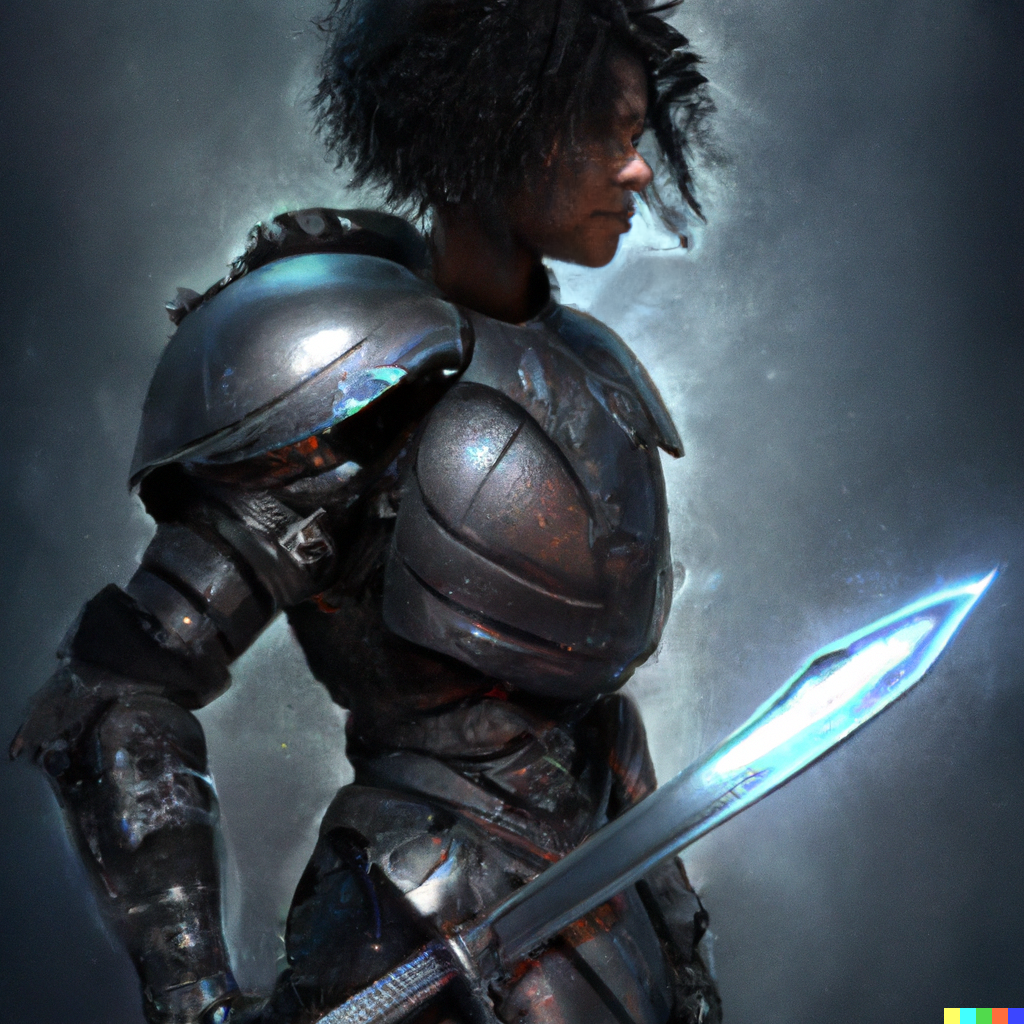
\includegraphics[width=\columnwidth]{equipment/armor}

    Most characters use armor to protect themselves. There are two kinds of armor: \glossterm{body armor}, such as full plate armor, and \glossterm{shields}.
    Body armor is worn on your body.
    You can only benefit from one body armor at a time.
    If you somehow wear multiple layers of body armor, the penalties stack and the benefits do not stack.
    A shield requires a free hand instead of being worn on the body.

    \subsection{Armor Mechanics}

        \subsubsection{Armor Usage Classes}\label{Armor Usage Classes}
            An armor's \glossterm{usage class} is a measure of how the armor is used, and how much effort is required to use it.
            It indicates whether armor, when used by a creature the armor is sized for, is considered light armor, medium armor, or heavy armor.

        \subsubsection{Armor Proficiency}\label{Armor Proficiency}
            Proficiency with armor is defined by the armor's usage class.
            If you wear or use armor you are not proficient with, it provides half its normal defense bonus.
            In addition, you apply that armor's \glossterm{encumbrance} as a penalty to your \glossterm{accuracy}.
            Since standard shields have no \glossterm{encumbrance}, you can use them without penalizing your attacks.

        \subsubsection{Getting Into And Out Of Armor}
            The time required to don armor depends on its type; see \trefnp{Donning Armor}. Donning and removing body armor and shields takes both hands.
            \parhead{Don} This column tells how long it takes a character to put the armor on. (One minute is 10 rounds.) Readying (strapping on) a shield is a \glossterm{free action}.
            \parhead{Remove} This column tells how long it takes to get the armor off.

            \begin{dtable}
                \lcaption{Donning Armor}
                \begin{dtabularx}{\columnwidth}{>{\lcol}X c c}
                    \tb{Armor Type}   & \tb{Don}          & \tb{Remove} \tableheaderrule
                    Light shield      & 1 free action     & 1 free action           \\
                    Medium shield     & 1 standard action & 1 standard action       \\
                    Tower shield      & 1 standard action & 1 standard action       \\
                    Light body armor  & 1 minute          & 1 minute\fn{1}          \\
                    Medium body armor & 4 minutes\fn{1}   & 1 minute\fn{1}          \\
                    Heavy body armor  & 4 minutes\fn{2}   & 1d4\plus1 minutes\fn{1} \\
                \end{dtabularx}
                1 If the character has some help, cut this time in half. A single character doing nothing else can help one or two adjacent characters. Two characters can't help each other don armor at the same time. \\
                2 The wearer must have help to don this armor.
            \end{dtable}

        \subsubsection{Weight and Size}
            The size category of body armor is the same as the size category of the creature it is sized for.
            Bucklers and standard shields are one size category smaller than the creature they are sized for, while tower shields are the same size category as the creature they are sized for.
            All armor and shields except for heavy body armor are \glossterm{lightweight} objects.
            In general, heavy body armor weighs so much that only creatures with a Strength of at least 1 can wear it (see \pcref{Weight Limits}).

    \subsection{Armor Table}
        \par Here is the format for armor entries (given as column headings on \trefnp{Armor and Shields}, below).

        \parhead{Defense} This value indicates how much the armor increases your Armor defense.

        \parhead{Damage Resistance} This value indicates how much the armor increases your \glossterm{damage resistance} (see \pcref{Damage Resistance}).

        \parhead{Encumbrance} This value indicates how much the armor increases your \glossterm{encumbrance}.
        You apply your encumbrance as a penalty to all Strength and Dexterity-based checks and skills.
        For details, see \pcref{Encumbrance}.

        \parhead{Speed} This penalty applies to speed with all of your \glossterm{movement modes} while wearing the armor.

        \parhead{Dex Bonus} This multiplier affects the contribution of your Dexterity to your Armor defense.
        It does not change any other effects that Dexterity has.

        \parhead{Item Rank (Cost)} The first value indicates the \glossterm{item rank} of the item (see \pcref{Item Ranks}).
        The second value in parentheses indicates the average cost to buy the item.
        Items crafted for unusually large or small creatures are more expensive.
        For each size category larger or smaller than Medium, the item's rank increases by one, which increases its price.

        \begin{dtable!*}
            \tablebookmark{Armor and Shields}{armor}
            \lcaption{Armor and Shields}
            \begin{dtabularx}{\textwidth}{l c c c c c >{\lcol}X c}
                \tb{Armor}            & \tb{Defense} & \tb{Damage Resistance} & \tb{Encumbrance} & \tb{Speed}   & \tb{Dex Bonus} & \tb{Material} & \tb{Item Rank (Cost)}  \tableheaderrule
                Light armor           &              &                        &                  &              &                &               &              \\
                \tind Leather         & \plus2       & \plus2                 & \tdash           & \tdash       & \tdash         & Leather       & 0 (10 gp)    \\
                \tind Studded leather & \plus2       & \plus3                 & \plus1           & \tdash       & \tdash         & Leather       & 1 (40 gp)    \\
                \tind Chain shirt     & \plus2       & \plus3                 & \plus1           & \tdash       & \tdash         & Metal         & 1 (40 gp)    \\
                \tind Buckler         & \plus1       & \tdash                 & \tdash           & \tdash       & \tdash         & Metal or wood & 0 (10 gp)    \\
                Medium armor          &              &                        &                  &              &                &               &              \\
                \tind Hide            & \plus3       & \plus3                 & \plus3           & \tdash  & \mult1/2       & Leather       & 1 (40 gp)    \\
                \tind Scale mail      & \plus3       & \plus5                 & \plus5           & \tdash  & \mult1/2       & Metal         & 1 (40 gp)    \\
                \tind Breastplate     & \plus3       & \plus6                 & \plus4           & \tdash  & \mult1/2       & Metal         & 2 (200 gp)   \\
                \tind Standard shield & \plus2       & \tdash                 & \tdash\fn{1}     & \tdash       & \mult1/2       & Metal or wood & 0 (10 gp)    \\
                Heavy armor           &              &                        &                  &              &                &               &              \\
                \tind Layered hide    & \plus4       & \plus8                 & \plus5           & \minus10 ft. & \mult0         & Leather       & 1 (40 gp)    \\
                \tind Plated mail     & \plus4       & \plus10                & \plus6           & \minus10 ft. & \mult0         & Metal         & 2 (200 gp)   \\
                \tind Full plate      & \plus4       & \plus12                & \plus6           & \minus10 ft. & \mult0         & Metal         & 3 (1,000 gp) \\
                \tind Tower shield    & \plus3\fn{2} & \tdash                 & \plus2\fn{1}     & \tdash       & \mult0         & Metal or wood & 1 (40 gp)    \\
                Extras                &              &                        &                  &              &                &               &              \\
                \tind Armor spikes    & \tdash       & \minus1                & \plus1           & \tdash       & \tdash         & Metal         & 0 (10 gp)    \\
                \tind Locked gauntlet & \tdash       & \tdash                 & Special          & \tdash       & \tdash         & Metal         & 0 (10 gp)    \\
                \tind Shield spikes   & \tdash       & \tdash                 & \plus1           & \tdash       & \tdash         & Metal         & 1 (40 gp)    \\
            \end{dtabularx}
            1 The hand holding the shield is not free, which may limit your actions. \\
            2 Tower shields improve your ability to take the \textit{total defense} action. See the description.
        \end{dtable!*}

    \subsection{Individual Armor Descriptions}
        Any special benefits or accessories to the types of armor found on \trefnp{Armor and Shields} are described below.
        \parhead{Armor Spikes} You can add armor spikes to any \glossterm{body armor}.
        Armor spikes are a \glossterm{weapon} that you can deal damage with (see \tref{Weapons}).
        \parhead{Breastplate} It comes with a helmet and greaves.
        \parhead{Buckler} This small metal shield is worn strapped to your forearm.
        You can treat the hand using a buckler as a \glossterm{free hand}.
        However, if you wield weapons or otherwise take actions using the arm bearing the buckler, you do not gain the buckler's defensive bonus during that phase.
        \par You can't bash someone with a buckler.
        \parhead{Chain Shirt} A chain shirt comes with a steel cap.
        \parhead{Full Plate} The suit includes gauntlets, heavy leather boots, a visored helmet, and a thick layer of padding that is worn underneath the armor. Each suit of full plate must be individually fitted to its owner by a master armorsmith, although a captured suit can be resized to fit a new owner with a day of work and a \glossterm{difficulty value} 10 Craft (metalworking) check. The new owner must still be of the same size category as the size category that the suit was designed for.
        \parhead{Shield, Standard, Wooden or Steel} You strap a shield to your forearm and grip it with your hand.
        A standard shield is so cumbersome that you can't use your shield hand for anything else.
        You can use a standard shield as a weapon (see \tref{Weapons}).
        However, you cannot use the \ability{offhand strike} ability to attack with a shield.
        \parhead{Shield, Tower} This massive shield is nearly as tall as an average human.
        When you take the \textit{total defense} action while wielding a tower shield, you gain a \plus2 bonus to Armor defense in addition to the normal bonuses from taking that action (see \pcref{Total Defense}).
        A tower shield is so cumbersome that you can't use your shield hand for anything else.
        You can use a tower shield as an \glossterm{exotic weapon} (see \tref{Exotic Weapons}).
        However, you cannot use the \ability{offhand strike} ability to attack with a shield.

        While wielding a tower shield, you take a \minus1 penalty to \glossterm{accuracy} because of the shield's unwieldy nature.
        \parhead{Shield Spikes} These spikes improve the effectiveness of a standard shield or tower shield when used as a weapon.
        You gain a \plus1d damage bonus with attacks using a spiked shield, and damage dealt by the strike is piercing damage in addition to any other damage types.
        You can't put spikes on a buckler.
        \parhead{Studded Leather} The studs on studded leather are made of metal, but this amount of metal is not generally enough to make the item count as being made of metal.
        Studded leather armor made with studs from special materials does not grant the wearer the properties of the special material.

    \subsection{Armor Special Materials}\label{Armor Special Materials}
        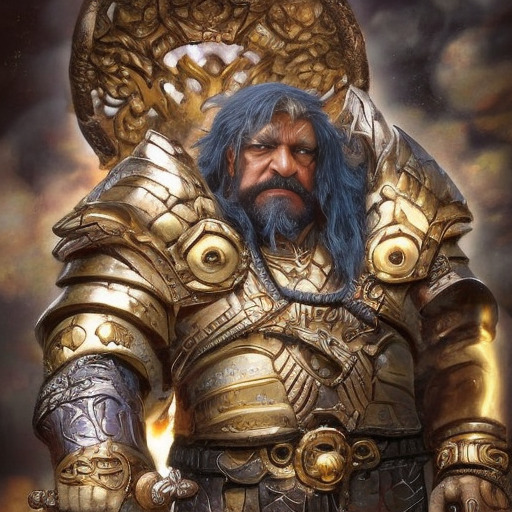
\includegraphics[width=\columnwidth]{equipment/armor special materials}
        Nonmagical body armor can be made from special materials that can alter the properties of the item.
        These special materials are described in \trefnp{Armor Special Materials}.
        The benefits here only apply to body armor that is fully made from the given special material.
        If you combine multiple special materials in any way, such as by wearing deepforged gauntlets with a mithral breastplate, you do not gain any benefits for having special materials.

        Body armor that is made from a special material cannot have any magic item properties, and cannot be chosen as a \glossterm{legacy item}.

        \begin{dtable!*}
            \lcaption{Armor Special Materials}
            \begin{dtabularx}{\textwidth}{l l l >{\ccol}X l l}
    \tb{Material}              & \tb{Damage Resistance} & \tb{Encumbrance} & \tb{Special Effect}                & \tb{Material} & \tb{Item Rank}              \tableheaderrule
    % metal high resistance, encum
    \tind Adamantine           & \mult4                 & \plus2           & \tdash                             & Metal         & \plus3  \\
    \tind Adamantine, pure     & \mult8                 & \plus2           & \tdash                             & Metal         & \plus5 \\
    % magic defense                                                          
    \tind Cold iron            & \mult1/2               & \tdash           & \plus1 defense vs magic            & Metal         & \plus2  \\
    \tind Cold iron, pure      & \mult1/2               & \tdash           & \plus2 defense vs magic            & Metal         & \plus4 \\
    % metal resistance                                                       
    \tind Deepforged           & \mult2                 & \tdash           & \tdash                             & Metal         & \plus2  \\
    \tind Deepforged, pure     & \mult4                 & \tdash           & \tdash                             & Metal         & \plus4 \\
    % metal crit resistance                                                  
    \tind Diamondsteel         & \tdash                 & \tdash           & \plus4 defense vs strike crits     & Metal         & \plus2  \\
    \tind Diamondsteel, pure   & \mult2                 & \tdash           & \plus4 defense vs crits            & Metal         & \plus4 \\
    % offset leather resistance, energy defense bonus                        
    \tind Dragonhide           & \mult3                 & \tdash           & Impervious to specific energy type & Leather       & \plus3  \\
    \tind Dragonhide, ancient  & \mult6                 & \tdash           & Immune to specific damage type     & Leather       & \plus5 \\
    % offset metal resistance, energy defense bonus                          
    \tind Dragonscale          & \mult3                 & \tdash           & Impervious to specific energy type & Metal         & \plus3  \\
    \tind Dragonscale, ancient & \mult6                 & \tdash           & Immune to specific energy type     & Metal         & \plus5 \\
    % leather resistance                                                     
    \tind Elvenweave           & \mult2                 & \tdash           & \tdash                             & Leather       & \plus2  \\
    \tind Elvenweave, pure     & \mult4                 & \tdash           & \tdash                             & Leather       & \plus4 \\
    % idk                                                                    
    \tind Ironwood             & \tdash                 & \tdash           & \tdash                             & Metal         & \plus1  \\
    % metal encumbrance reduction                                            
    \tind Mithral              & \tdash                 & \minus2          & \tdash                             & Metal         & \plus2  \\
    \tind Mithral, pure        & \mult2                 & \minus3          & Improve Dex multiplier                 & Metal         & \plus4 \\
    % metal resistance, recovery, encumbrance penalty                        
    \tind Starmetal            & \mult2                 & \plus2           & Recover damage resistance                & Metal         & \plus2  \\
    \tind Starmetal, pure      & \mult4                 & \plus2           & Recover damage resistance                & Metal         & \plus4 \\
\end{dtabularx}
        \end{dtable!*}

        \parhead{Adamantine} Adamantine armor increases the \glossterm{encumbrance} of the armor by 2, but it multiplies the \glossterm{damage resistance} provided by the armor by 4.
        The armor's item rank is increased by 3, which increases the typical cost to buy the item (see \pcref{Item Ranks}).

        \parhead{Adamantine, Pure} Pure adamantine armor increases the \glossterm{encumbrance} of the armor by 2, but it multiplies the \glossterm{damage resistance} provided by the armor by 8.
        The armor's item rank is increased by 5, which increases the typical cost to buy the item (see \pcref{Item Ranks}).

        \parhead{Cold Iron} Cold iron armor provides half the normal \glossterm{damage resistance}.
        In exchange, it grants a \plus1 bonus to your defenses against \magical abilities.
        The armor's item rank is increased by 2, which increases the typical cost to buy the item (see \pcref{Item Ranks}).

        \parhead{Cold Iron, Pure} Pure cold iron armor provides half the normal \glossterm{damage resistance}.
        In exchange, it grants a \plus2 bonus to your defenses against \magical abilities.
        The armor's item rank is increased by 4, which increases the typical cost to buy the item (see \pcref{Item Ranks}).

        \parhead{Deepforged} Deepforged body armor multiplies the \glossterm{damage resistance} provided by the armor by 2.
        The armor's item rank is increased by 2, which increases the typical cost to buy the item (see \pcref{Item Ranks}).

        \parhead{Deepforged, Pure} Pure deepforged body armor multiplies the \glossterm{damage resistance} provided by the armor by 4.
        The armor's item rank is increased by 4, which increases the typical cost to buy the item (see \pcref{Item Ranks}).

        \parhead{Diamondsteel} Diamondsteel body armor grants you a \plus4 bonus to your defenses when determining whether a \glossterm{strike} gets a \glossterm{critical hit} against you instead of a normal hit.
        The armor's item rank is increased by 2, which increases the typical cost to buy the item (see \pcref{Item Ranks}).

        \parhead{Diamondsteel, Pure} Pure diamondsteel body armor grants you a \plus4 bonus to your defenses when determining whether any attack gets a \glossterm{critical hit} against you instead of a normal hit.
        In addition, it multiplies the \glossterm{damage resistance} provided by the armor by 2.
        The armor's item rank is increased by 4, which increases the typical cost to buy the item (see \pcref{Item Ranks}).

        \parhead{Dragonhide} Dragonhide body armor multiplies the \glossterm{damage resistance} provided by the armor by 3.
        In addition, each dragonhide body armor is made from the hide of a particular type of dragon.
        You are \trait{impervious} to damage of the type dealt by that dragon's breath weapon (see \tref{Dragon Types}).
        The armor's item rank is increased by 3, which increases the typical cost to buy the item (see \pcref{Item Ranks}).

        \parhead{Dragonhide, Ancient} Ancient dragonhide body armor multiplies the \glossterm{damage resistance} provided by the armor by 6.
        In addition, each ancient dragonhide body armor is made from the hide of a particular type of dragon.
        You are \trait{immune} to damage of the type dealt by that dragon's breath weapon (see \tref{Dragon Types}).
        The armor's item rank is increased by 5, which increases the typical cost to buy the item (see \pcref{Item Ranks}).

        \parhead{Dragonscale} Dragonscale body armor multiplies the \glossterm{damage resistance} provided by the armor by 3.
        It is not considered to be metal, which may affect abilities like the \spell{heat metal} spell.
        In addition, each dragonscale body armor is made from the scales of a particular type of dragon.
        You are \trait{impervious} to damage of the type dealt by that dragon's breath weapon (see \tref{Dragon Types}).
        The armor's item rank is increased by 3, which increases the typical cost to buy the item (see \pcref{Item Ranks}).

        \parhead{Dragonscale, Ancient} Ancient dragonscale body armor multiplies the \glossterm{damage resistance} provided by the armor by 6.
        It is not considered to be metal, which may affect abilities like the \spell{heat metal} spell.
        In addition, each ancient dragonscale body armor is made from the scales of a particular type of dragon.
        You are \trait{immune} to damage of the type dealt by that dragon's breath weapon (see \tref{Dragon Types}).
        The armor's item rank is increased by 5, which increases the typical cost to buy the item (see \pcref{Item Ranks}).

        \parhead{Elvenweave} Elvenweave body armor multiplies the \glossterm{damage resistance} provided by the armor by 2.
        The armor's item rank is increased by 2, which increases the typical cost to buy the item (see \pcref{Item Ranks}).

        \parhead{Ironwood} The most common special material is ironwood, which is made from wood magically treated using the \spell{ironwood} ritual to be as strong as steel. Ironwood armor functions exactly like armor of the same type, except that it is made of wood.
        The armor's item rank is increased by 1, which increases the typical cost to buy the item (see \pcref{Item Ranks}).

        \parhead{Mithral} Mithral body armor reduces the \glossterm{encumbrance} of the armor by 2.
        The armor's item rank is increased by 2, which increases the typical cost to buy the item (see \pcref{Item Ranks}).

        \parhead{Mithral, Pure} Pure mithral body armor multiplies the \glossterm{damage resistance} provided by the armor by 2.
        In addition, it reduces the \glossterm{encumbrance} of the armor by 3, and it increases the contribution of your Dexterity to your Armor defense relative to the normal limit for that type of armor.
        A multiplier of \mult1/2 becomes \mult1, and a multiplier of \mult0 becomes a \mult1/2.
        The armor's item rank is increased by 4, which increases the typical cost to buy the item (see \pcref{Item Ranks}).

        \parhead{Starmetal} Starmetal body armor multiplies the \glossterm{damage resistance} provided by the armor by 2.
        In addition, it increases the \glossterm{encumbrance} of the armor by 2.
        When you use the \ability{recover} ability while wearing starmetal body armor, you also regain an amount of \glossterm{damage resistance} equal to half the damage resistance provided by the armor.
        This effect is \abilitytag{Swift}, like the \ability{recover} ability.
        The armor's item rank is increased by 2, which increases the typical cost to buy the item (see \pcref{Item Ranks}).

        \parhead{Starmetal, Pure} Pure starmetal body armor multiplies the \glossterm{damage resistance} provided by the armor by 4.
        In addition, it increases the \glossterm{encumbrance} of the armor by 2.
        When you use the \ability{recover} ability while wearing starmetal body armor, you also regain an amount of \glossterm{damage resistance} equal to half the damage resistance provided by the armor.
        This effect is \abilitytag{Swift}, like the \ability{recover} ability.
        The armor's item rank is increased by 4, which increases the typical cost to buy the item (see \pcref{Item Ranks}).

\newpage
\section{Magic Armor}
    Magic body armor must be worn to gain its effects, while magic shields must be wielded.

    \subsection{Magic Armor and Damage Resistance}
        While you are attuned to magical body armor, that armor gains a multiplier to the damage resistance it provides.
        This multiplier does not apply to any special properties the armor might have, such as a magic bonus to your damage resistance.
        It only applies to the normal damage resistance normally provided by body armor of that type.
        The magnitude of the multiplier is based on the magic item's rank, as listed below.

        \begin{itemize}
            \item Rank 0--3: \mult1
            \item Rank 4: \mult2
            \item Rank 5: \mult3
            \item Rank 6: \mult4
            \item Rank 7: \mult6
        \end{itemize}


    \input{generated/armor_table.tex}

    \input{generated/armor.tex}

\newpage
\section{Magic Apparel}
    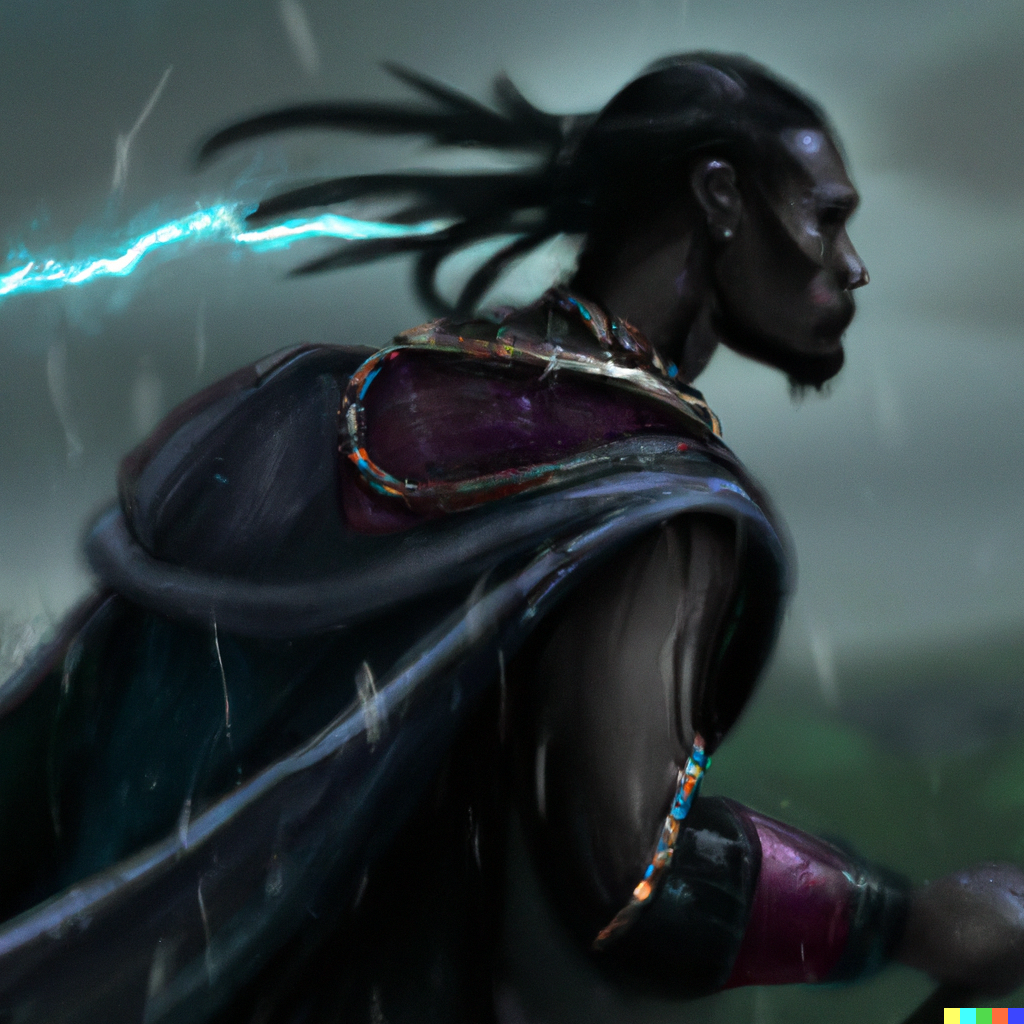
\includegraphics[width=\columnwidth]{equipment/magic apparel}
    Magic apparel items must be worn to gain their effects.

    \subsection{Body Slots}
        The main limiting factor on how many items you can have equipped is your attunement points, not the physical location of your items on your body.
        However, there are limits to how many items you can wear of the same type, as described below.
        For item types not listed here, use reasonable judgment about what would be plausible.
        \begin{itemize}
            \item Amulet: Up to 3
            \item Belt: Up to 3
            \item Boots: Up to 1
            \item Circlet: Up to 1
            \item Cloak: Up to 3
            \item Gauntlets: Up to 1 (separate from gloves)
            \item Gloves: Up to 1 (separate from gauntlets)
            \item Rings: Up to 5 per hand
        \end{itemize}

    
\begin{longtablewrapper}
\begin{longtable}{p{15em} p{3em} p{6em} p{25em} p{3em}}

\lcaption{Apparel Items} \\
\tb{Name} & \tb{Level} & \tb{Typical Price} & \tb{Description} & \tb{Page} \tableheaderrule
Bracers of Archery & \nth{1} & 50 gp & Grants bow proficiency & \pageref{item:Bracers of Archery} \\
Belt of Healing & \nth{2} & 125 gp & Grants healing & \pageref{item:Belt of Healing} \\
Boots of the Winterlands & \nth{2} & 125 gp & Eases travel in cold areas & \pageref{item:Boots of the Winterlands} \\
Bracers of Armor & \nth{2} & 125 gp & Grants invisible armor & \pageref{item:Bracers of Armor} \\
Gauntlets of Improvisation & \nth{2} & 125 gp & Grants \plus1d damage with improvised weapons & \pageref{item:Gauntlets of Improvisation} \\
Ring of Elemental Endurance & \nth{2} & 125 gp & Grants tolerance of temperature extremes & \pageref{item:Ring of Elemental Endurance} \\
Shield of Bashing & \nth{2} & 125 gp & Grants \plus2 power & \pageref{item:Shield of Bashing} \\
Torchlight Gloves & \nth{2} & 125 gp & Sheds light as a torch & \pageref{item:Torchlight Gloves} \\
Ocular Circlet & \nth{3} & 250 gp & Can allow you to see at a distance & \pageref{item:Ocular Circlet} \\
Ring of Nourishment & \nth{3} & 250 gp & Provides food and water & \pageref{item:Ring of Nourishment} \\
Boots of Earth's Embrace & \nth{4} & 500 gp & Grants immunity to forced movement & \pageref{item:Boots of Earth's Embrace} \\
Boots of Elvenkind & \nth{4} & 500 gp & Grants \plus2 Stealth & \pageref{item:Boots of Elvenkind} \\
Circlet of Persuasion & \nth{4} & 500 gp & Grants \plus2 Persuasion & \pageref{item:Circlet of Persuasion} \\
Gauntlet of the Ram & \nth{4} & 500 gp & Knocks back foe when used to strike & \pageref{item:Gauntlet of the Ram} \\
Mask of Water Breathing & \nth{4} & 500 gp & Allows breathing water like air & \pageref{item:Mask of Water Breathing} \\
Throwing Gloves & \nth{4} & 500 gp & Allows throwing any item accurately & \pageref{item:Throwing Gloves} \\
Acid Coated & \nth{5} & 800 gp & Deals acid damage to anything it touches & \pageref{item:Acid Coated} \\
Amulet of Translocation & \nth{5} & 800 gp & Grants ability to teleport up to 30 feet & \pageref{item:Amulet of Translocation} \\
Circlet of Blasting & \nth{5} & 800 gp & Can blast foe with fire & \pageref{item:Circlet of Blasting} \\
Hidden Armor & \nth{5} & 800 gp & Can look like normal clothing & \pageref{item:Hidden Armor} \\
Protective Armor & \nth{5} & 800 gp & Grants \plus1 Armor defense & \pageref{item:Protective Armor} \\
Protective Shield & \nth{5} & 800 gp & Grants \plus1 Armor defense & \pageref{item:Protective Shield} \\
Shield of Arrow Catching & \nth{5} & 800 gp & Redirects small nearby projectiles to hit you & \pageref{item:Shield of Arrow Catching} \\
Shield of Arrow Deflection & \nth{5} & 800 gp & Blocks small projectiles & \pageref{item:Shield of Arrow Deflection} \\
Translocation & \nth{5} & 800 gp & Grants ability to teleport up to 30 feet & \pageref{item:Translocation} \\
Agile & \nth{6} & 1,200 gp & Grants \plus2 Reflex defense & \pageref{item:Agile} \\
Amulet of Health & \nth{6} & 1,200 gp & Grants 2 additional hit points & \pageref{item:Amulet of Health} \\
Amulet of Nondetection & \nth{6} & 1,200 gp & Grants \plus4 to defenses against detection & \pageref{item:Amulet of Nondetection} \\
Boots of Speed & \nth{6} & 1,200 gp & Increases speed by ten feet & \pageref{item:Boots of Speed} \\
Featherlight Armor & \nth{6} & 1,200 gp & Reduces encumbrance by 1 & \pageref{item:Featherlight Armor} \\
Fortified & \nth{6} & 1,200 gp & Grants \plus2 Fortitude defense & \pageref{item:Fortified} \\
Quilled Cloak & \nth{6} & 1,200 gp & Deals damage to creatures that grapple you & \pageref{item:Quilled Cloak} \\
Willguard & \nth{6} & 1,200 gp & Grants \plus2 Mental defense & \pageref{item:Willguard} \\
Anchoring & \nth{7} & 1,800 gp & Protects you from most forced movement attacks & \pageref{item:Anchoring} \\
Armor of Fortification & \nth{7} & 1,800 gp & Reduces critical hits from strikes & \pageref{item:Armor of Fortification} \\
Boots of Water Walking & \nth{7} & 1,800 gp & Allows walking on liquids & \pageref{item:Boots of Water Walking} \\
Boots of the Skydancer & \nth{7} & 1,800 gp & Can walk on air & \pageref{item:Boots of the Skydancer} \\
Bracers of Archery, Greater & \nth{7} & 1,800 gp & Grants bow proficiency, \plus1 ranged accuracy & \pageref{item:Bracers of Archery, Greater} \\
Bracers of Repulsion & \nth{7} & 1,800 gp & Can knock nearby creatures back & \pageref{item:Bracers of Repulsion} \\
Crown of Lightning & \nth{7} & 1,800 gp & Continuously damages nearby enemies & \pageref{item:Crown of Lightning} \\
Gauntlet of the Ram, Greater & \nth{7} & 1,800 gp & Knocks back foe farther when use to strike & \pageref{item:Gauntlet of the Ram, Greater} \\
Gauntlets of Improvisation, Greater & \nth{7} & 1,800 gp & Grants \plus2d damage with improvised weapons & \pageref{item:Gauntlets of Improvisation, Greater} \\
Gloves of Spell Investment & \nth{7} & 1,800 gp & Can invest a spell to cast later & \pageref{item:Gloves of Spell Investment} \\
Hexward Amulet & \nth{7} & 1,800 gp & Grants \plus1 defenses against targeted magical attacks & \pageref{item:Hexward Amulet} \\
Lifekeeping Belt & \nth{7} & 1,800 gp & Grants \plus1 bonus to \glossterm{vital rolls} & \pageref{item:Lifekeeping Belt} \\
Ring of Sustenance & \nth{7} & 1,800 gp & Provides food, water, and rest & \pageref{item:Ring of Sustenance} \\
Amulet of Mighty Fists & \nth{8} & 2,750 gp & Grants \plus2 power with natural and unarmed attacks & \pageref{item:Amulet of Mighty Fists} \\
Armor of Energy Resistance & \nth{8} & 2,750 gp & Reduces energy damage & \pageref{item:Armor of Energy Resistance} \\
Armor of Invulnerability & \nth{8} & 2,750 gp & Reduces physical damage & \pageref{item:Armor of Invulnerability} \\
Assassin's Cloak & \nth{8} & 2,750 gp & Grants invisibility while inactive & \pageref{item:Assassin's Cloak} \\
Avian Cloak & \nth{8} & 2,750 gp & Grants a glide speed & \pageref{item:Avian Cloak} \\
Belt of Healing, Greater & \nth{8} & 2,750 gp & Grants more healing & \pageref{item:Belt of Healing, Greater} \\
Boots of Gravitation & \nth{8} & 2,750 gp & Redirects personal gravity & \pageref{item:Boots of Gravitation} \\
Cloak of Mist & \nth{8} & 2,750 gp & Fills nearby area with fog & \pageref{item:Cloak of Mist} \\
Ring of Protection & \nth{8} & 2,750 gp & Grants \plus1 to Armor and Reflex defenses & \pageref{item:Ring of Protection} \\
Shield of Boulder Catching & \nth{8} & 2,750 gp & Redirects large nearby projectiles to hit you & \pageref{item:Shield of Boulder Catching} \\
Shield of Boulder Deflection & \nth{8} & 2,750 gp & Can block large projectiles & \pageref{item:Shield of Boulder Deflection} \\
Crown of Flame & \nth{9} & 4,000 gp & Grants nearby allies immunity to fire damage & \pageref{item:Crown of Flame} \\
Greatreach Bracers & \nth{9} & 4,000 gp & Increases reach by five feet & \pageref{item:Greatreach Bracers} \\
Hidden Armor, Greater & \nth{9} & 4,000 gp & Can look and sound like normal clothing & \pageref{item:Hidden Armor, Greater} \\
Mask of Air & \nth{9} & 4,000 gp & Allows breathing in any environment & \pageref{item:Mask of Air} \\
Ocular Circlet, Greater & \nth{9} & 4,000 gp & Can allow you to see at a greater distance & \pageref{item:Ocular Circlet, Greater} \\
Ring of Angel's Grace & \nth{9} & 4,000 gp & Grants \plus2 Mental and slows falls & \pageref{item:Ring of Angel's Grace} \\
Boots of Speed, Greater & \nth{10} & 6,500 gp & Increases speed by twenty feet & \pageref{item:Boots of Speed, Greater} \\
Circlet of Blasting, Greater & \nth{10} & 6,500 gp & Can blast foe with intense fire & \pageref{item:Circlet of Blasting, Greater} \\
Crater Boots & \nth{10} & 6,500 gp & Deals your falling damage to enemies & \pageref{item:Crater Boots} \\
Titan Gauntlets & \nth{10} & 6,500 gp & Grants \plus2 \glossterm{mundane} power & \pageref{item:Titan Gauntlets} \\
Winged Boots & \nth{10} & 6,500 gp & Grants limited flight & \pageref{item:Winged Boots} \\
Amulet of Translocation, Greater & \nth{11} & 10,000 gp & Grants ability to teleport up to 100 feet & \pageref{item:Amulet of Translocation, Greater} \\
Crown of Thunder & \nth{11} & 10,000 gp & Continously deafens nearby enemies & \pageref{item:Crown of Thunder} \\
Shield of Arrow Catching, Greater & \nth{11} & 10,000 gp & Selectively redirects small nearby projectiles to hit you & \pageref{item:Shield of Arrow Catching, Greater} \\
Shield of Bashing, Greater & \nth{11} & 10,000 gp & Grants \plus4 power & \pageref{item:Shield of Bashing, Greater} \\
Translocation, Greater & \nth{11} & 10,000 gp & Grants ability to teleport up to 100 feet & \pageref{item:Translocation, Greater} \\
Amulet of the Planes & \nth{12} & 16,000 gp & Aids travel with \ritual{plane shift} & \pageref{item:Amulet of the Planes} \\
Armor of Fortification, Mystic & \nth{12} & 16,000 gp & Reduces critical hits from all attacks & \pageref{item:Armor of Fortification, Mystic} \\
Boots of Freedom & \nth{12} & 16,000 gp & Grants immunity to almost all mobility restrictions & \pageref{item:Boots of Freedom} \\
Featherlight Armor, Greater & \nth{12} & 16,000 gp & Reduces encumbrance by 2 & \pageref{item:Featherlight Armor, Greater} \\
Greater Quilled Cloak & \nth{12} & 16,000 gp & Deals more damage to creatures that grapple you & \pageref{item:Greater Quilled Cloak} \\
Ring of Energy Resistance & \nth{12} & 16,000 gp & Reduces energy damage & \pageref{item:Ring of Energy Resistance} \\
Seven League Boots & \nth{12} & 16,000 gp & Teleport seven leages with a step & \pageref{item:Seven League Boots} \\
Shield of Mystic Reflection & \nth{12} & 16,000 gp & React to reflect magical attacks & \pageref{item:Shield of Mystic Reflection} \\
Anchoring, Greater & \nth{13} & 25,000 gp & Protects you from all forced movement and teleportation attacks & \pageref{item:Anchoring, Greater} \\
Assassin's Cloak, Greater & \nth{13} & 25,000 gp & Grants longer invisibility while inactive & \pageref{item:Assassin's Cloak, Greater} \\
Boots of the Skydancer, Greater & \nth{13} & 25,000 gp & description & \pageref{item:Boots of the Skydancer, Greater} \\
Crown of Frost & \nth{13} & 25,000 gp & Continuously damages nearby enemies & \pageref{item:Crown of Frost} \\
Gloves of Spell Investment, Greater & \nth{13} & 25,000 gp & Can invest two spells to cast later & \pageref{item:Gloves of Spell Investment, Greater} \\
Hexproof Amulet, Greater & \nth{13} & 25,000 gp & Grants \plus2 defenses against targeted magical attacks & \pageref{item:Hexproof Amulet, Greater} \\
Lifekeeping Belt, Greater & \nth{13} & 25,000 gp & Grants \plus2 bonus to \glossterm{vital rolls} & \pageref{item:Lifekeeping Belt, Greater} \\
Vanishing Cloak & \nth{13} & 25,000 gp & Can teleport a short distance and grant invisibility & \pageref{item:Vanishing Cloak} \\
Amulet of Nondetection, Greater & \nth{14} & 37,000 gp & Grants \plus8 to defenses against detection & \pageref{item:Amulet of Nondetection, Greater} \\
Armor of Energy Resistance, Greater & \nth{14} & 37,000 gp & Significantly reduces energy damage & \pageref{item:Armor of Energy Resistance, Greater} \\
Armor of Invulnerability & \nth{14} & 37,000 gp & Significantly reduces physical damage & \pageref{item:Armor of Invulnerability} \\
Belt of Healing, Supreme & \nth{14} & 37,000 gp & Grants more healing & \pageref{item:Belt of Healing, Supreme} \\
Boots of Speed, Supreme & \nth{14} & 37,000 gp & Increases speed by thirty feet & \pageref{item:Boots of Speed, Supreme} \\
Protective Armor, Greater & \nth{14} & 37,000 gp & Grants \plus2 Armor defense & \pageref{item:Protective Armor, Greater} \\
Protective Shield, Greater & \nth{14} & 37,000 gp & Grants \plus2 Armor defense & \pageref{item:Protective Shield, Greater} \\
Shield of Arrow Deflection, Greater & \nth{14} & 37,000 gp & Blocks small projectiles & \pageref{item:Shield of Arrow Deflection, Greater} \\
Agile, Greater & \nth{15} & 55,000 gp & Grants \plus4 Reflex defense & \pageref{item:Agile, Greater} \\
Amulet of Health, Greater & \nth{15} & 55,000 gp & Grants 4 additional hit points & \pageref{item:Amulet of Health, Greater} \\
Armor of Fortification, Greater & \nth{15} & 55,000 gp & Drastically reduces critical hits from strikes & \pageref{item:Armor of Fortification, Greater} \\
Bracers of Repulsion, Greater & \nth{15} & 55,000 gp & Can knock many nearby creatures back & \pageref{item:Bracers of Repulsion, Greater} \\
Fortified, Greater & \nth{15} & 55,000 gp & Grants \plus4 Fortitude defense & \pageref{item:Fortified, Greater} \\
Ring of Regeneration & \nth{15} & 55,000 gp & Automatically removes vital wounds & \pageref{item:Ring of Regeneration} \\
Willguard, Greater & \nth{15} & 55,000 gp & Grants \plus4 Mental defense & \pageref{item:Willguard, Greater} \\
Amulet of Mighty Fists, Greater & \nth{16} & 85,000 gp & Grants \plus4 power with natural and unarmed attacks & \pageref{item:Amulet of Mighty Fists, Greater} \\
Astral Boots & \nth{16} & 85,000 gp & Allows teleporting instead of moving & \pageref{item:Astral Boots} \\
Circlet of Blasting, Supreme & \nth{16} & 85,000 gp & Can blast foe with supremely intense fire & \pageref{item:Circlet of Blasting, Supreme} \\
Cloak of Mist, Greater & \nth{16} & 85,000 gp & Fills nearby area with thick fog & \pageref{item:Cloak of Mist, Greater} \\
Ring of Protection, Greater & \nth{16} & 85,000 gp & Grants \plus2 to Armor and Reflex defenses & \pageref{item:Ring of Protection, Greater} \\
Amulet of Translocation, Supreme & \nth{17} & 125,000 gp & Grants ability to teleport up to 300 feet & \pageref{item:Amulet of Translocation, Supreme} \\
Greatreach Bracers, Greater & \nth{17} & 125,000 gp & Increases reach by ten feet & \pageref{item:Greatreach Bracers, Greater} \\
Shield of Boulder Deflection, Greater & \nth{17} & 125,000 gp & Blocks large projectiles & \pageref{item:Shield of Boulder Deflection, Greater} \\
Translocation, Supreme & \nth{17} & 125,000 gp & Grants ability to teleport up to 300 feet & \pageref{item:Translocation, Supreme} \\
Featherlight Armor, Supreme & \nth{18} & 190,000 gp & Reduces encumbrance by 2 & \pageref{item:Featherlight Armor, Supreme} \\
Supreme Quilled Cloak & \nth{18} & 190,000 gp & Deals even more damage to creatures that grapple you & \pageref{item:Supreme Quilled Cloak} \\
Hexproof Amulet, Supreme & \nth{19} & 280,000 gp & Grants \plus3 defenses against targeted magical attacks & \pageref{item:Hexproof Amulet, Supreme} \\
Lifekeeping Belt, Supreme & \nth{19} & 280,000 gp & Grants \plus3 bonus to \glossterm{vital rolls} & \pageref{item:Lifekeeping Belt, Supreme} \\
Titan Gauntlets, Greater & \nth{19} & 280,000 gp & Grants \plus4 \glossterm{mundane} power & \pageref{item:Titan Gauntlets, Greater} \\
Armor of Energy Resistance, Supreme & \nth{20} & 400,000 gp & Drastically reduces energy damage & \pageref{item:Armor of Energy Resistance, Supreme} \\
Armor of Invulnerability, Greater & \nth{20} & 400,000 gp & Drastically reduces physical damage & \pageref{item:Armor of Invulnerability, Greater} \\
Shield of Bashing, Supreme & \nth{20} & 400,000 gp & Grants \plus6 power & \pageref{item:Shield of Bashing, Supreme} \\

\end{longtable}
\end{longtablewrapper}


    \lowercase{\hypertarget{item:Amulet of Mighty Fists}{}}\label{item:Amulet of Mighty Fists}
\hypertarget{item:Amulet of Mighty Fists}{\subsubsection{Amulet of Mighty Fists\hfill\nth{6}}}
You gain a \plus1d bonus to \glossterm{strike damage} with \glossterm{unarmed attacks} and natural weapons.
\parhead*{Tags} \glossterm{Enhancement}
\parhead*{Materials} Jewelry
\lowercase{\hypertarget{item:Amulet of Mighty Fists, Greater}{}}\label{item:Amulet of Mighty Fists, Greater}
\hypertarget{item:Amulet of Mighty Fists, Greater}{\subsubsection{Amulet of Mighty Fists, Greater\hfill\nth{14}}}
You gain a \plus2d bonus to \glossterm{strike damage} with \glossterm{unarmed attacks} and natural weapons.
\parhead*{Tags} \glossterm{Enhancement}
\parhead*{Materials} Jewelry
\lowercase{\hypertarget{item:Armor of Energy Resistance}{}}\label{item:Armor of Energy Resistance}
\hypertarget{item:Armor of Energy Resistance}{\subsubsection{Armor of Energy Resistance\hfill\nth{4}}}
You have \glossterm{damage reduction} equal to the item's \glossterm{power} against \glossterm{energy damage}.
Whenever you resist energy with this item, it sheds light as a torch until the end of the next round.
The color of the light depends on the energy damage resisted: blue for cold, yellow for electricity, red for fire, and brown for sonic.
\parhead*{Tags} \glossterm{Shielding}
\parhead*{Materials} Bone, metal
\lowercase{\hypertarget{item:Armor of Energy Resistance, Greater}{}}\label{item:Armor of Energy Resistance, Greater}
\hypertarget{item:Armor of Energy Resistance, Greater}{\subsubsection{Armor of Energy Resistance, Greater\hfill\nth{12}}}
This item functions like the \mitem{armor of energy resistance} item, except that the damage reduction is equal to twice the item's \glossterm{power}.
\parhead*{Tags} \glossterm{Shielding}
\parhead*{Materials} Bone, metal
\lowercase{\hypertarget{item:Armor of Fortification}{}}\label{item:Armor of Fortification}
\hypertarget{item:Armor of Fortification}{\subsubsection{Armor of Fortification\hfill\nth{7}}}
You gain a \plus5 bonus to defenses when determining whether a \glossterm{strike} gets a \glossterm{critical hit} against you instead of a normal hit.
\parhead*{Tags} \glossterm{Imbuement}
\parhead*{Materials} Bone, metal
\lowercase{\hypertarget{item:Armor of Fortification, Greater}{}}\label{item:Armor of Fortification, Greater}
\hypertarget{item:Armor of Fortification, Greater}{\subsubsection{Armor of Fortification, Greater\hfill\nth{15}}}
This item functions like the \mitem{armor of fortification} item, except that the bonus increases to \plus10.
\parhead*{Tags} \glossterm{Imbuement}
\parhead*{Materials} Bone, metal
\lowercase{\hypertarget{item:Armor of Fortification, Mystic}{}}\label{item:Armor of Fortification, Mystic}
\hypertarget{item:Armor of Fortification, Mystic}{\subsubsection{Armor of Fortification, Mystic\hfill\nth{12}}}
This item functions like the \mitem{armor of fortification} item, except that it applies against all attacks instead of only against; \glossterm{strikes}.
\parhead*{Tags} \glossterm{Imbuement}
\parhead*{Materials} Bone, metal
\lowercase{\hypertarget{item:Armor of Invulnerability}{}}\label{item:Armor of Invulnerability}
\hypertarget{item:Armor of Invulnerability}{\subsubsection{Armor of Invulnerability\hfill\nth{8}}}
You have \glossterm{damage reduction} equal to this item's \glossterm{power} against damage from \glossterm{physical attacks}.
\parhead*{Tags} \glossterm{Shielding}
\parhead*{Materials} Bone, metal
\lowercase{\hypertarget{item:Armor of Invulnerability, Greater}{}}\label{item:Armor of Invulnerability, Greater}
\hypertarget{item:Armor of Invulnerability, Greater}{\subsubsection{Armor of Invulnerability, Greater\hfill\nth{16}}}
This item functions like the \mitem{armor of invulnerability} item, except that the damage reduction is equal to twice the item's \glossterm{power}.
You have \glossterm{damage reduction} equal to the item's \glossterm{power} against damage from \glossterm{physical attacks}.
\parhead*{Tags} \glossterm{Shielding}
\parhead*{Materials} Bone, metal
\lowercase{\hypertarget{item:Armor of Magic Resistance}{}}\label{item:Armor of Magic Resistance}
\hypertarget{item:Armor of Magic Resistance}{\subsubsection{Armor of Magic Resistance\hfill\nth{14}}}
You have \glossterm{magic resistance} equal to 5 + the item's \glossterm{power}.
\parhead*{Tags} \glossterm{Shielding}
\parhead*{Materials} Bone, metal
\lowercase{\hypertarget{item:Assassin's Cloak}{}}\label{item:Assassin's Cloak}
\hypertarget{item:Assassin's Cloak}{\subsubsection{Assassin's Cloak\hfill\nth{7}}}
At the end of each round, if you took no actions that round, you become \glossterm{invisible} until the end of the next round.
\parhead*{Tags} \glossterm{Glamer}
\parhead*{Materials} Textiles
\lowercase{\hypertarget{item:Assassin's Cloak, Greater}{}}\label{item:Assassin's Cloak, Greater}
\hypertarget{item:Assassin's Cloak, Greater}{\subsubsection{Assassin's Cloak, Greater\hfill\nth{17}}}
At the end of each round, if you did not attack a creature that round, you become \glossterm{invisible} until the end of the next round.
\parhead*{Tags} \glossterm{Glamer}
\parhead*{Materials} Textiles
\lowercase{\hypertarget{item:Astral Boots}{}}\label{item:Astral Boots}
\hypertarget{item:Astral Boots}{\subsubsection{Astral Boots\hfill\nth{16}}}
Whenever you move, you can teleport the same distance instead.
This does not change the total distance you can move, but you can teleport in any direction, even vertically.
You cannot teleport to locations you do not have \glossterm{line of sight} and \glossterm{line of effect} to.
\parhead*{Tags} \glossterm{Teleportation}
\parhead*{Materials} Bone, leather, metal
\lowercase{\hypertarget{item:Belt of Healing}{}}\label{item:Belt of Healing}
\hypertarget{item:Belt of Healing}{\subsubsection{Belt of Healing\hfill\nth{1}}}
When you use the \textit{recover} action, you heal \plus1d hit points.
\parhead*{Tags} \glossterm{Life}
\parhead*{Materials} Leather, textiles
\lowercase{\hypertarget{item:Belt of Healing, Greater}{}}\label{item:Belt of Healing, Greater}
\hypertarget{item:Belt of Healing, Greater}{\subsubsection{Belt of Healing, Greater\hfill\nth{8}}}
When you use the \textit{recover} action, you heal \plus2d hit points.
\parhead*{Tags} \glossterm{Life}
\parhead*{Materials} Leather, textiles
\lowercase{\hypertarget{item:Belt of Heroic Recovery}{}}\label{item:Belt of Heroic Recovery}
\hypertarget{item:Belt of Heroic Recovery}{\subsubsection{Belt of Heroic Recovery\hfill\nth{6}}}
% TODO: timing?
As an \glossterm{immediate action} when you get a \glossterm{critical hit}, you can take the \textit{recover} action.
\parhead*{Tags} \glossterm{Life}
\parhead*{Materials} Leather, textiles
\lowercase{\hypertarget{item:Boots of Earth's Embrace}{}}\label{item:Boots of Earth's Embrace}
\hypertarget{item:Boots of Earth's Embrace}{\subsubsection{Boots of Earth's Embrace\hfill\nth{4}}}
While you are standing on solid ground, you are immune to effects that would force you to move.
This does not protect you from other effects of those attacks, such as damage.
\parhead*{Tags} \glossterm{Earth}, \glossterm{Enhancement}
\parhead*{Materials} Bone, leather, metal
\lowercase{\hypertarget{item:Boots of Freedom}{}}\label{item:Boots of Freedom}
\hypertarget{item:Boots of Freedom}{\subsubsection{Boots of Freedom\hfill\nth{6}}}
You are immune to effects that restrict your mobility.
This removes all penalties you would suffer for acting underwater, except for those relating to using ranged weapons.
This does not prevent you from being \grappled, but you gain a \plus10 bonus to your defense against \glossterm{grapple} attacks.
\parhead*{Tags} \glossterm{Imbuement}
\parhead*{Materials} Bone, leather, metal
\lowercase{\hypertarget{item:Boots of Freedom, Greater}{}}\label{item:Boots of Freedom, Greater}
\hypertarget{item:Boots of Freedom, Greater}{\subsubsection{Boots of Freedom, Greater\hfill\nth{12}}}
These boots function like \mitem{boots of freedom}, except that you are also immune to being \grappled.
\parhead*{Tags} \glossterm{Imbuement}
\parhead*{Materials} Bone, leather, metal
\lowercase{\hypertarget{item:Boots of Gravitation}{}}\label{item:Boots of Gravitation}
\hypertarget{item:Boots of Gravitation}{\subsubsection{Boots of Gravitation\hfill\nth{8}}}
While these boots are within 5 feet of a solid surface, gravity pulls you towards the solid surface closest to your boots rather than in the normal direction.
This can allow you to walk easily on walls or even ceilings.
\parhead*{Tags} \glossterm{Imbuement}
\parhead*{Materials} Bone, leather, metal
\lowercase{\hypertarget{item:Boots of Speed}{}}\label{item:Boots of Speed}
\hypertarget{item:Boots of Speed}{\subsubsection{Boots of Speed\hfill\nth{5}}}
You gain a \plus10 foot bonus to your speed in all your movement modes, up to a maximum of double your normal speed.
\parhead*{Tags} \glossterm{Temporal}
\parhead*{Materials} Bone, leather, metal
\lowercase{\hypertarget{item:Boots of Speed, Greater}{}}\label{item:Boots of Speed, Greater}
\hypertarget{item:Boots of Speed, Greater}{\subsubsection{Boots of Speed, Greater\hfill\nth{13}}}
You gain a \plus30 foot bonus to your speed in all your movement modes, up to a maximum of double your normal speed.
\parhead*{Tags} \glossterm{Temporal}
\parhead*{Materials} Bone, leather, metal
\lowercase{\hypertarget{item:Boots of Water Walking}{}}\label{item:Boots of Water Walking}
\hypertarget{item:Boots of Water Walking}{\subsubsection{Boots of Water Walking\hfill\nth{7}}}
You treat the surface of all liquids as if they were firm ground.
Your feet hover about an inch above the liquid's surface, allowing you to traverse dangerous liquids without harm as long as the surface is calm.
If you are below the surface of the liquid, you rise towards the surface at a rate of 60 feet per round.
Thick liquids, such as mud and lava, may cause you to rise more slowly.
\parhead*{Tags} \glossterm{Imbuement}
\parhead*{Materials} Bone, leather, metal
\lowercase{\hypertarget{item:Boots of the Winterlands}{}}\label{item:Boots of the Winterlands}
\hypertarget{item:Boots of the Winterlands}{\subsubsection{Boots of the Winterlands\hfill\nth{2}}}
You can travel across snow and ice without slipping or suffering movement penalties for the terrain.
% TODO: degree symbol?
In addition, the boots keep you warn, protecting you in environments as cold as \minus50 Fahrenheit.
\parhead*{Tags} \glossterm{Enhancement}
\parhead*{Materials} Bone, leather, metal
\lowercase{\hypertarget{item:Bracers of Archery}{}}\label{item:Bracers of Archery}
\hypertarget{item:Bracers of Archery}{\subsubsection{Bracers of Archery\hfill\nth{1}}}
You are proficient with bows.
\parhead*{Tags} \glossterm{Enhancement}
\parhead*{Materials} Bone, leather, metal, wood
\lowercase{\hypertarget{item:Bracers of Armor}{}}\label{item:Bracers of Armor}
\hypertarget{item:Bracers of Armor}{\subsubsection{Bracers of Armor\hfill\nth{2}}}
You gain a \plus2 bonus to Armor defense.
The protection from these bracers is treated as body armor, and it does not stack with any other body armor you wear.
\parhead*{Tags} \glossterm{Shielding}
\parhead*{Materials} Bone, leather, metal, wood
\lowercase{\hypertarget{item:Bracers of Repulsion}{}}\label{item:Bracers of Repulsion}
\hypertarget{item:Bracers of Repulsion}{\subsubsection{Bracers of Repulsion\hfill\nth{4}}}
Whenever a creature hits you with a melee \glossterm{strike} during the \glossterm{action phase},
you can spend an \glossterm{action point} to use this item as an \glossterm{immediate action}.
If you do, you make a \glossterm{shove} attack against that creature during the \glossterm{delayed action phase}, using this item's power in place of your Strength.
\parhead*{Tags} \glossterm{Telekinesis}
\parhead*{Materials} Bone, leather, metal, wood
\lowercase{\hypertarget{item:Bracers of Repulsion, Greater}{}}\label{item:Bracers of Repulsion, Greater}
\hypertarget{item:Bracers of Repulsion, Greater}{\subsubsection{Bracers of Repulsion, Greater\hfill\nth{11}}}
This item functions like the \mitem{bracers of repulsion} item, except that it does not cost an action point to use.
\parhead*{Tags} \glossterm{Telekinesis}
\parhead*{Materials} Bone, leather, metal, wood
\lowercase{\hypertarget{item:Cloak of Mist}{}}\label{item:Cloak of Mist}
\hypertarget{item:Cloak of Mist}{\subsubsection{Cloak of Mist\hfill\nth{8}}}
Fog constantly fills an \areamed radius emanation from you.
This fog does not fully block sight, but it provides \concealment.
If a 5-foot square of fog takes fire damage equal to half this item's \glossterm{power}, the fog disappears from that area until the end of the next round.
\parhead*{Tags} \glossterm{Fog}, \glossterm{Manifestation}
\parhead*{Materials} Textiles
\lowercase{\hypertarget{item:Cloak of Mist, Greater}{}}\label{item:Cloak of Mist, Greater}
\hypertarget{item:Cloak of Mist, Greater}{\subsubsection{Cloak of Mist, Greater\hfill\nth{16}}}
A thick fog constantly fills an \areamed radius emanation from you.
This fog completely blocks sight beyond 10 feet.
Within that range, it still provides \concealment.
If a 5-foot square of fog takes fire damage equal to this item's \glossterm{power}, the fog disappears from that area until the end of the next round.
\parhead*{Tags} \glossterm{Fog}, \glossterm{Manifestation}
\parhead*{Materials} Textiles
\lowercase{\hypertarget{item:Crown of Flame}{}}\label{item:Crown of Flame}
\hypertarget{item:Crown of Flame}{\subsubsection{Crown of Flame\hfill\nth{5}}}
This crown is continuously on fire.
The flame sheds light as a torch.
You and all allies within an \arealarge radius emanation from you are immune to fire damage.
\parhead*{Tags} \glossterm{Fire}
\parhead*{Materials} Bone, metal
\lowercase{\hypertarget{item:Crown of Frost}{}}\label{item:Crown of Frost}
\hypertarget{item:Crown of Frost}{\subsubsection{Crown of Frost\hfill\nth{11}}}
At the end of each \glossterm{action phase}, you make a Power vs. Fortitude attack against all enemies within an \areamed radius emanation from you.
A hit deals cold \glossterm{standard damage} \minus3d.
Each creature that takes damage in this way is \fatigued until the end of the next round.
\parhead*{Tags} \glossterm{Cold}
\parhead*{Materials} Bone, metal
\lowercase{\hypertarget{item:Crown of Lightning}{}}\label{item:Crown of Lightning}
\hypertarget{item:Crown of Lightning}{\subsubsection{Crown of Lightning\hfill\nth{7}}}
This crown continuously crackles with electricity.
The constant sparks shed light as a torch.
At the end of each \glossterm{action phase}, you make a Power vs. Reflex attack against all enemies within an \areamed radius emanation from you.
A hit deals electricity \glossterm{standard damage} \minus3d.
\parhead*{Tags} \glossterm{Electricity}
\parhead*{Materials} Bone, metal
\lowercase{\hypertarget{item:Crown of Thunder}{}}\label{item:Crown of Thunder}
\hypertarget{item:Crown of Thunder}{\subsubsection{Crown of Thunder\hfill\nth{9}}}
The crown constantly emits a low-pitched rumbling.
To you and your allies, the sound is barely perceptible.
However, all enemies within an \arealarge radius emanation from you hear the sound as a deafening, continuous roll of thunder.
The noise blocks out all other sounds quieter than thunder, causing them to be \deafened while they remain in the area and until the end of the next round after they leave.
\parhead*{Tags} \glossterm{Sonic}
\parhead*{Materials} Bone, metal
\lowercase{\hypertarget{item:Featherlight Armor}{}}\label{item:Featherlight Armor}
\hypertarget{item:Featherlight Armor}{\subsubsection{Featherlight Armor\hfill\nth{4}}}
This armor's \glossterm{encumbrance penalty} is reduced by 2.
\parhead*{Tags} \glossterm{Enhancement}
\parhead*{Materials} Bone, metal
\lowercase{\hypertarget{item:Featherlight Armor, Greater}{}}\label{item:Featherlight Armor, Greater}
\hypertarget{item:Featherlight Armor, Greater}{\subsubsection{Featherlight Armor, Greater\hfill\nth{10}}}
This armor's \glossterm{encumbrance penalty} is reduced by 4.
\parhead*{Tags} \glossterm{Enhancement}
\parhead*{Materials} Bone, metal
\lowercase{\hypertarget{item:Gauntlet of the Ram}{}}\label{item:Gauntlet of the Ram}
\hypertarget{item:Gauntlet of the Ram}{\subsubsection{Gauntlet of the Ram\hfill\nth{2}}}
If you hit on a \glossterm{strike} with this gauntlet during the \glossterm{action phse}, you can attempt to \glossterm{shove} your foe during the \glossterm{delayed action phase}.
Making a strike with this gauntlet is equivalent to an \glossterm{unarmed attack}.
You do not need to move with your foe to push it back the full distance.
\parhead*{Tags} \glossterm{Telekinesis}
\parhead*{Materials} Bone, metal, wood
\lowercase{\hypertarget{item:Gauntlet of the Ram, Greater}{}}\label{item:Gauntlet of the Ram, Greater}
\hypertarget{item:Gauntlet of the Ram, Greater}{\subsubsection{Gauntlet of the Ram, Greater\hfill\nth{7}}}
This item functions like the \mitem{gauntlet of the ram}, except that you gain a bonus to the \glossterm{shove} attack equal to the damage you dealt with the \glossterm{strike}.
\parhead*{Tags} \glossterm{Telekinesis}
\parhead*{Materials} Bone, metal, wood
\lowercase{\hypertarget{item:Gauntlets of Improvisation}{}}\label{item:Gauntlets of Improvisation}
\hypertarget{item:Gauntlets of Improvisation}{\subsubsection{Gauntlets of Improvisation\hfill\nth{2}}}
You gain a \plus1d bonus to damage with \glossterm{improvised weapons}.
\parhead*{Tags} \glossterm{Enhancement}
\parhead*{Materials} Bone, metal, wood
\lowercase{\hypertarget{item:Gauntlets of Improvisation, Greater}{}}\label{item:Gauntlets of Improvisation, Greater}
\hypertarget{item:Gauntlets of Improvisation, Greater}{\subsubsection{Gauntlets of Improvisation, Greater\hfill\nth{7}}}
This item functions like the \mitem{gauntlets of improvisation}, except that the damage bonus is increased to \plus2d.
\parhead*{Tags} \glossterm{Enhancement}
\parhead*{Materials} Bone, metal, wood
\lowercase{\hypertarget{item:Greatreach Bracers}{}}\label{item:Greatreach Bracers}
\hypertarget{item:Greatreach Bracers}{\subsubsection{Greatreach Bracers\hfill\nth{9}}}
Your \glossterm{reach} is increased by 5 feet.
\parhead*{Tags} \glossterm{Imbuement}
\parhead*{Materials} Bone, leather, metal, wood
\lowercase{\hypertarget{item:Greatreach Bracers, Greater}{}}\label{item:Greatreach Bracers, Greater}
\hypertarget{item:Greatreach Bracers, Greater}{\subsubsection{Greatreach Bracers, Greater\hfill\nth{17}}}
Your \glossterm{reach} is increased by 10 feet.
\parhead*{Tags} \glossterm{Imbuement}
\parhead*{Materials} Bone, leather, metal, wood
\lowercase{\hypertarget{item:Hexproof Cloak}{}}\label{item:Hexproof Cloak}
\hypertarget{item:Hexproof Cloak}{\subsubsection{Hexproof Cloak\hfill\nth{18}}}
All \glossterm{magical} abilities that target you directly fail to affect you.
This does not protect you from abilities that affect an area.
\parhead*{Tags} \glossterm{Thaumaturgy}
\parhead*{Materials} Textiles
\lowercase{\hypertarget{item:Hexward Cloak}{}}\label{item:Hexward Cloak}
\hypertarget{item:Hexward Cloak}{\subsubsection{Hexward Cloak\hfill\nth{10}}}
You gain a \plus5 bonus to defenses against \glossterm{magical} abilities that target you directly.
This does not protect you from abilities that affect an area.
\parhead*{Tags} \glossterm{Thaumaturgy}
\parhead*{Materials} Textiles
\lowercase{\hypertarget{item:Hidden Armor}{}}\label{item:Hidden Armor}
\hypertarget{item:Hidden Armor}{\subsubsection{Hidden Armor\hfill\nth{4}}}
As a standard action, you can use this item.
If you do, it appears to change shape and form to assume the shape of a normal set of clothing.
You may choose the design of the clothing.
The item retains all of its properties, including weight and sound, while disguised in this way.
Only its visual appearance is altered.
Alternately, you may return the armor to its original appearance.
\parhead*{Tags} \glossterm{Glamer}
\parhead*{Materials} Bone, metal
\lowercase{\hypertarget{item:Hidden Armor, Greater}{}}\label{item:Hidden Armor, Greater}
\hypertarget{item:Hidden Armor, Greater}{\subsubsection{Hidden Armor, Greater\hfill\nth{9}}}
This item functions like the \mitem{hidden armor} item, except that the item also makes sound appropriate to its disguised form while disguised.
\parhead*{Tags} \glossterm{Alteration}
\parhead*{Materials} Bone, metal
\lowercase{\hypertarget{item:Mask of Air}{}}\label{item:Mask of Air}
\hypertarget{item:Mask of Air}{\subsubsection{Mask of Air\hfill\nth{9}}}
If you breathe through this mask, you breathe in clean, fresh air, regardless of your environment.
This can protect you from inhaled poisons and similar effects.
\parhead*{Tags} \glossterm{Imbuement}
\parhead*{Materials} Textiles
\lowercase{\hypertarget{item:Mask of Water Breathing}{}}\label{item:Mask of Water Breathing}
\hypertarget{item:Mask of Water Breathing}{\subsubsection{Mask of Water Breathing\hfill\nth{4}}}
You can breathe water through this mask as easily as a human breaths air.
This does not grant you the ability to breathe other liquids.
\parhead*{Tags} \glossterm{Imbuement}
\parhead*{Materials} Textiles
\lowercase{\hypertarget{item:Ring of Elemental Endurance}{}}\label{item:Ring of Elemental Endurance}
\hypertarget{item:Ring of Elemental Endurance}{\subsubsection{Ring of Elemental Endurance\hfill\nth{2}}}
You can exist comfortably in conditions between \minus50 and 140 degrees Fahrenheit without any ill effects.
You suffer the normal penalties in temperatures outside of that range.
\parhead*{Tags} \glossterm{Shielding}
\parhead*{Materials} Bone, jewelry, metal, wood
\lowercase{\hypertarget{item:Ring of Energy Resistance}{}}\label{item:Ring of Energy Resistance}
\hypertarget{item:Ring of Energy Resistance}{\subsubsection{Ring of Energy Resistance\hfill\nth{6}}}
You have \glossterm{damage reduction} equal to the ring's \glossterm{power} against \glossterm{energy damage}.
Whenever you resist energy with this ability, the ring sheds light as a torch until the end of the next round.
The color of the light depends on the energy damage resisted: blue for cold, yellow for electricity, red for fire, and brown for sonic.
\parhead*{Tags} \glossterm{Shielding}
\parhead*{Materials} Bone, jewelry, metal, wood
\lowercase{\hypertarget{item:Ring of Energy Resistance, Greater}{}}\label{item:Ring of Energy Resistance, Greater}
\hypertarget{item:Ring of Energy Resistance, Greater}{\subsubsection{Ring of Energy Resistance, Greater\hfill\nth{14}}}
This item functions like the \mitem{ring of energy resistance}, except that the damage reduction is equal to twice the item's \glossterm{power}.
\parhead*{Tags} \glossterm{Shielding}
\parhead*{Materials} Bone, jewelry, metal, wood
\lowercase{\hypertarget{item:Ring of Nourishment}{}}\label{item:Ring of Nourishment}
\hypertarget{item:Ring of Nourishment}{\subsubsection{Ring of Nourishment\hfill\nth{3}}}
You continuously gain nourishment, and no longer need to eat or drink.
This ring must be worn for 24 hours before it begins to work.
\parhead*{Tags} \glossterm{Creation}
\parhead*{Materials} Bone, jewelry, metal, wood
\lowercase{\hypertarget{item:Ring of Protection}{}}\label{item:Ring of Protection}
\hypertarget{item:Ring of Protection}{\subsubsection{Ring of Protection\hfill\nth{8}}}
You gain a \plus1 bonus to Armor defense.
\parhead*{Tags} \glossterm{Shielding}
\parhead*{Materials} Bone, jewelry, metal, wood
\lowercase{\hypertarget{item:Ring of Regeneration}{}}\label{item:Ring of Regeneration}
\hypertarget{item:Ring of Regeneration}{\subsubsection{Ring of Regeneration\hfill\nth{11}}}
At the end of each \glossterm{action phase}, you heal hit points equal to this item's \glossterm{power}.
Only damage taken while wearing the ring can be healed in this way.
\parhead*{Tags} \glossterm{Life}
\parhead*{Materials} Bone, jewelry, metal, wood
\lowercase{\hypertarget{item:Ring of Sustenance}{}}\label{item:Ring of Sustenance}
\hypertarget{item:Ring of Sustenance}{\subsubsection{Ring of Sustenance\hfill\nth{7}}}
You continuously gain nourishment, and no longer need to eat or drink.
In addition, you need only one-quarter your normal amount of sleep (or similar activity, such as elven trance) each day.
The ring must be worn for 24 hours before it begins to work.
\parhead*{Tags} \glossterm{Creation}, \glossterm{Temporal}
\parhead*{Materials} Bone, jewelry, metal, wood
\lowercase{\hypertarget{item:Seven League Boots}{}}\label{item:Seven League Boots}
\hypertarget{item:Seven League Boots}{\subsubsection{Seven League Boots\hfill\nth{12}}}
As a standard action, you can spend an \glossterm{action point} to use this item.
If you do, you teleport exactly 25 miles in a direction you specify.
If this would place you within a solid object or otherwise impossible space, the boots will shunt you up to 1,000 feet in any direction to the closest available space.
If there is no available space within 1,000 feet of your intended destination, the effect fails and you take \glossterm{standard damage} \minus1d.
\parhead*{Tags} \glossterm{Teleportation}
\parhead*{Materials} Bone, leather, metal
\lowercase{\hypertarget{item:Shield of Arrow Catching}{}}\label{item:Shield of Arrow Catching}
\hypertarget{item:Shield of Arrow Catching}{\subsubsection{Shield of Arrow Catching\hfill\nth{5}}}
Whenever a creature within a \areamed radius emanation from you would be attacked by a ranged weapon, the attack is redirected to target you instead.
Resolve the attack as if it had initially targeted you, except that the attack is not affected by cover or concealment.
This item can only affect projectiles and thrown objects that are Small or smaller.
\parhead*{Tags} \glossterm{Telekinesis}
\parhead*{Materials} Bone, metal, wood
\lowercase{\hypertarget{item:Shield of Arrow Catching, Greater}{}}\label{item:Shield of Arrow Catching, Greater}
\hypertarget{item:Shield of Arrow Catching, Greater}{\subsubsection{Shield of Arrow Catching, Greater\hfill\nth{10}}}
This item functions like the \mitem{shield of arrow catching} item, except that it affects a \arealarge radius from you.
In addition, you may choose to exclude creature from this item's effect, allowing projectiles to target nearby foes normally.
\parhead*{Tags} \glossterm{Telekinesis}
\parhead*{Materials} Bone, metal, wood
\lowercase{\hypertarget{item:Shield of Arrow Deflection}{}}\label{item:Shield of Arrow Deflection}
\hypertarget{item:Shield of Arrow Deflection}{\subsubsection{Shield of Arrow Deflection\hfill\nth{2}}}
As an \glossterm{immediate action} when you are attacked by a ranged \glossterm{strike}, you can use this item.
If you do, you gain a \plus5 bonus to Armor defense against the attack.
You must be aware of the attack to deflect it in this way.
This item can only affect projectiles and thrown objects that are Small or smaller.
\parhead*{Tags} \glossterm{Telekinesis}
\parhead*{Materials} Bone, metal, wood
\lowercase{\hypertarget{item:Shield of Arrow Deflection, Greater}{}}\label{item:Shield of Arrow Deflection, Greater}
\hypertarget{item:Shield of Arrow Deflection, Greater}{\subsubsection{Shield of Arrow Deflection, Greater\hfill\nth{12}}}
This item functions like the \mitem{shield of arrow deflection} item, except that the defense bonus increases to \plus10.
\parhead*{Tags} \glossterm{Telekinesis}
\parhead*{Materials} Bone, metal, wood
\lowercase{\hypertarget{item:Shield of Bashing}{}}\label{item:Shield of Bashing}
\hypertarget{item:Shield of Bashing}{\subsubsection{Shield of Bashing\hfill\nth{2}}}
% Should this be strike damage?
You gain a \plus1d bonus to damage with \glossterm{physical attacks} using this shield.
\parhead*{Tags} \glossterm{Enhancement}
\parhead*{Materials} Bone, metal, wood
\lowercase{\hypertarget{item:Shield of Bashing, Greater}{}}\label{item:Shield of Bashing, Greater}
\hypertarget{item:Shield of Bashing, Greater}{\subsubsection{Shield of Bashing, Greater\hfill\nth{11}}}
% Should this be strike damage?
You gain a \plus2d bonus to damage with \glossterm{physical attacks} using this shield.
\parhead*{Tags} \glossterm{Enhancement}
\parhead*{Materials} Bone, metal, wood
\lowercase{\hypertarget{item:Shield of Boulder Catching}{}}\label{item:Shield of Boulder Catching}
\hypertarget{item:Shield of Boulder Catching}{\subsubsection{Shield of Boulder Catching\hfill\nth{8}}}
This item functions like the \mitem{shield of arrow catching} item, except that it can affect projectile and thrown objects of up to Large size.
\parhead*{Tags} \glossterm{Telekinesis}
\parhead*{Materials} Bone, metal, wood
\lowercase{\hypertarget{item:Shield of Boulder Deflection}{}}\label{item:Shield of Boulder Deflection}
\hypertarget{item:Shield of Boulder Deflection}{\subsubsection{Shield of Boulder Deflection\hfill\nth{6}}}
This item functions like the \mitem{shield of arrow deflection} item, except that it can affect projectiles and thrown objects of up to Large size.
\parhead*{Tags} \glossterm{Telekinesis}
\parhead*{Materials} Bone, metal, wood
\lowercase{\hypertarget{item:Shield of Mystic Reflection}{}}\label{item:Shield of Mystic Reflection}
\hypertarget{item:Shield of Mystic Reflection}{\subsubsection{Shield of Mystic Reflection\hfill\nth{12}}}
As an \glossterm{immediate action} when you are targeted by a targeted \glossterm{magical} ability, you can spend an \glossterm{action point} to use this ability.
If you do, the ability targets the creature using the ability instead of you.
Any other targets of the ability are affected normally.
\parhead*{Tags} \glossterm{Thaumaturgy}
\parhead*{Materials} Bone, metal, wood
\lowercase{\hypertarget{item:Throwing Gloves}{}}\label{item:Throwing Gloves}
\hypertarget{item:Throwing Gloves}{\subsubsection{Throwing Gloves\hfill\nth{4}}}
% TODO: reference basic "not designed to be thrown" mechanics?
You can throw any item as if it was designed to be thrown.
This does not improve your ability to throw items designed to be thrown, such as darts.
\parhead*{Tags} \glossterm{Enhancement}
\parhead*{Materials} Leather
\lowercase{\hypertarget{item:Torchlight Gloves}{}}\label{item:Torchlight Gloves}
\hypertarget{item:Torchlight Gloves}{\subsubsection{Torchlight Gloves\hfill\nth{2}}}
These gloves shed light as a torch.
As a \glossterm{standard action}, you may choose to suppress or resume the light from either or both gloves.
\parhead*{Tags} \glossterm{Figment}, \glossterm{Light}
\parhead*{Materials} Leather
\lowercase{\hypertarget{item:Vanishing Cloak}{}}\label{item:Vanishing Cloak}
\hypertarget{item:Vanishing Cloak}{\subsubsection{Vanishing Cloak\hfill\nth{8}}}
As a standard action, you can spend an \glossterm{action point} to use this item.
If you do, you teleport to an unoccupied location within \rngmed range of your original location.
In addition, you become \glossterm{invisible} unitl the end of the next round.
If your intended destination is invalid, or if your teleportation otherwise fails, you still become invisible.
\parhead*{Tags} \glossterm{Glamer}, \glossterm{Teleportation}
\parhead*{Materials} Textiles
\lowercase{\hypertarget{item:Winged Boots}{}}\label{item:Winged Boots}
\hypertarget{item:Winged Boots}{\subsubsection{Winged Boots\hfill\nth{10}}}
You gain a \glossterm{fly speed} equal to your land speed.
However, the boots are not strong enough to keep you aloft indefinitely.
At the end of each round, if you are not standing on solid ground, the magic of the boots fails and you fall normally.
The boots begin working again at the end of the next round, even if you have not yet hit the ground.
\parhead*{Tags} \glossterm{Imbuement}
\parhead*{Materials} Bone, leather, metal

\newpage
\section{Magic Implements}\label{Implements}
    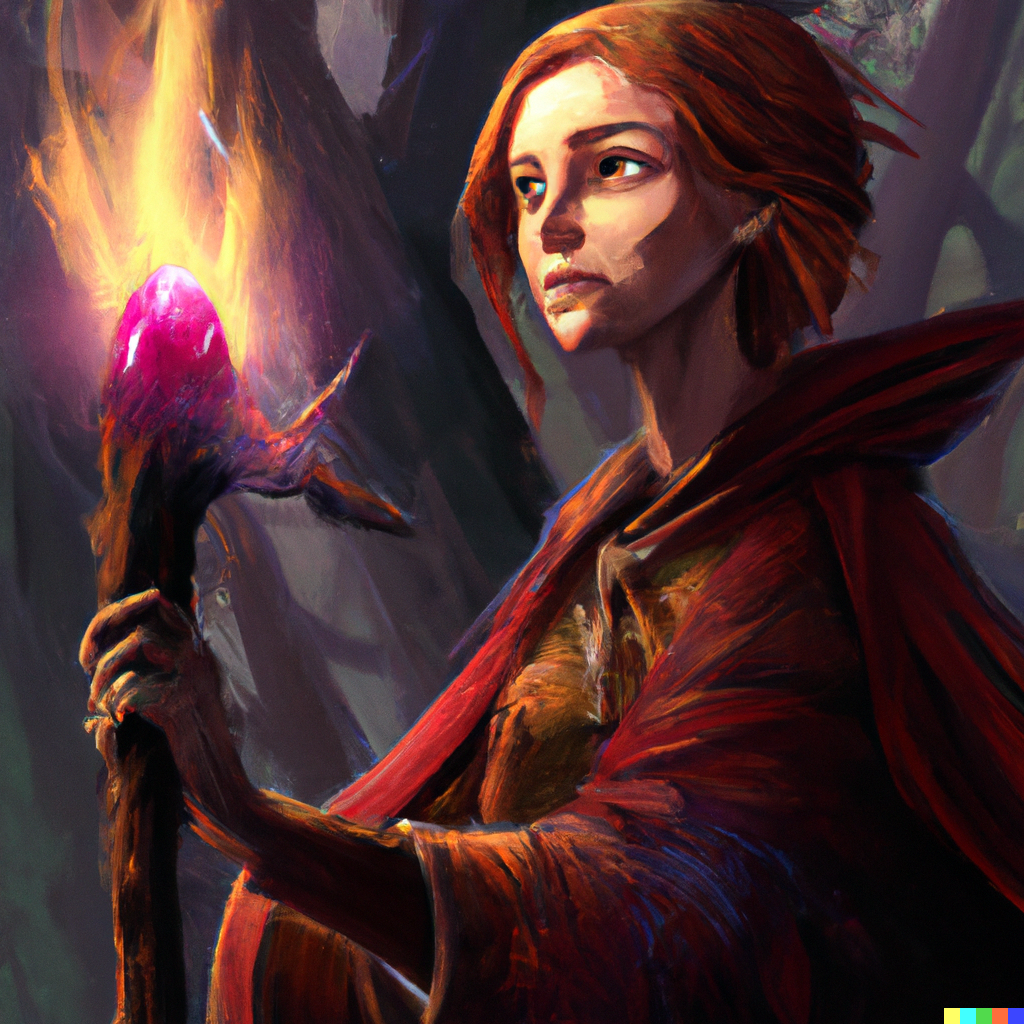
\includegraphics[width=\columnwidth]{equipment/magic implements}
    Implements can take many forms: staffs, wands, holy symbols, and more.
    Like magic weapons, magic implements must be wielded to gain their effects.
    However, while weapons are used to deal damage to enemies, implements are used to cast spells.

    \parhead{Somatic Components} While wielding an implement, you may gesture with it and channel magic through it.
    These qualify as somatic components for the purpose of casting spells.
    This does not remove the possibility of \glossterm{somatic component failure}.

    \subsection{Implement Types}

        \subsubsection{Holy Symbols}

            \parhead{Physical Description} A typical holy symbol is a no larger than 4 inches in each dimension and can be easily held in the palm of a hand.
            Most holy symbols are metal, but they can be made from wood, bone, or even more exotic materials, depending on the deity they symbolize.

            \parhead{Special Rules} All holy symbols are implements for divine spells.
            Most holy symbols are designed to be worn as an amulet in addition to being held in the hand.
            A magical holy symbol grants its magical abilities if it is either worn as an amulet or held in the hand.

        \subsubsection{Staffs}

            \parhead{Physical Description} A typical staff is 3 feet to 7 feet long and 2 inches to 3 inches thick, weighing about 5 pounds.
            Most staffs are wood, but a rare few are bone, metal, or even glass.
            Staffs often have a gem or some device at their tip or are shod in metal at one or both ends.

            Staffs are often decorated with carvings or runes.
            Long staffs are quarterstaffs.
            They must be held in two hands, and can be used to attack like any other quarterstaff.
            Short staffs resemble thin clubs.
            They can be held in one hand, but are not suitable for combat and are treated as \glossterm{improvised weapons} if used to attack.
            A typical staff has 20 \glossterm{hit points} and a sunder \glossterm{difficulty value} of 10.

        \subsubsection{Wands}

            \parhead{Physical Description} A typical wand is 6 inches to 12 inches long and about 1/4 inch thick, and usually weighs no more than 1 ounce.
            Most wands are wood, but some are bone.
            A rare few are metal, glass, or even ceramic, but these are quite exotic.
            Occasionally, a wand has a gem or some device at its tip, and most are decorated with carvings or runes.
            A typical wand has 5 \glossterm{hit points} and a sunder \glossterm{difficulty value} of 5.

    
\begin{longtabuwrapper}
\begin{longtabu}{l l X l}
\lcaption{Implement Items} \\
\tb{Name} & \tb{Level} & \tb{Description} & \tb{Page} \\
\bottomrule
Wand of Spellpower & \nth{4} & Grants \plus1 power with a single spell & \pageref{item:Wand of Spellpower} \\
Staff of Transit & \nth{5} & Doubles your teleportation distance & \pageref{item:Staff of Transit} \\
Spellfeeding Staff & \nth{6} & Heals you when casting spells & \pageref{item:Spellfeeding Staff} \\
Staff of Spellpower & \nth{8} & Grants \plus1 power with spells & \pageref{item:Staff of Spellpower} \\
Staff of Sympathetic Shielding & \nth{8} & Shields you when shielding others & \pageref{item:Staff of Sympathetic Shielding} \\
Wand of Precision & \nth{8} & Grants \plus1 accuracy with a single spell & \pageref{item:Wand of Precision} \\
Staff of Precision & \nth{10} & Grants \plus1 accuracy with spells & \pageref{item:Staff of Precision} \\
Wand of Spellpower, Greater & \nth{10} & Grants \plus2 power with a single spell & \pageref{item:Wand of Spellpower, Greater} \\
Spellfeeding Staff, Greater & \nth{14} & Greatly heals you when casting spells & \pageref{item:Spellfeeding Staff, Greater} \\
Staff of Spellpower, Greater & \nth{14} & Grants \plus2 power with spells & \pageref{item:Staff of Spellpower, Greater} \\
Wand of Precision, Greater & \nth{14} & Grants \plus2 accuracy with a single spell & \pageref{item:Wand of Precision, Greater} \\
Greater Staff of Precision & \nth{16} & Grants \plus2 accuracy with spells & \pageref{item:Greater Staff of Precision} \\
Wand of Spellpower, Supreme & \nth{16} & Grants \plus3 power with a single spell & \pageref{item:Wand of Spellpower, Supreme} \\
Staff of Spellpower, Supreme & \nth{20} & Grants \plus3 power with spells & \pageref{item:Staff of Spellpower, Supreme} \\
\end{longtabu}
\end{longtabuwrapper}


    
\lowercase{\hypertarget{item:Extending Staff}{}}\label{item:Extending Staff}
\hypertarget{item:Extending Staff}{\subsubsection{Extending Staff\hfill\nth{10} (6,500 gp)}}

You double the range of your \glossterm{magical} abilities.



\vspace{0.25em}
\spelltwocol{\textbf{Type}: Staff}{}
\textbf{Materials}: Bone, wood


\lowercase{\hypertarget{item:Extending Staff, Greater}{}}\label{item:Extending Staff, Greater}
\hypertarget{item:Extending Staff, Greater}{\subsubsection{Extending Staff, Greater\hfill\nth{19} (280,000 gp)}}

You triple the range of your \glossterm{magical} abilities.



\vspace{0.25em}
\spelltwocol{\textbf{Type}: Staff}{}
\textbf{Materials}: Bone, wood


\lowercase{\hypertarget{item:Protective Staff}{}}\label{item:Protective Staff}
\hypertarget{item:Protective Staff}{\subsubsection{Protective Staff\hfill\nth{5} (800 gp)}}

You gain a \plus1 \glossterm{magic bonus} to Armor defense.



\vspace{0.25em}
\spelltwocol{\textbf{Type}: Staff}{}
\textbf{Materials}: Bone, wood


\lowercase{\hypertarget{item:Protective Staff, Greater}{}}\label{item:Protective Staff, Greater}
\hypertarget{item:Protective Staff, Greater}{\subsubsection{Protective Staff, Greater\hfill\nth{14} (37,000 gp)}}

You gain a \plus2 \glossterm{magic bonus} to Armor defense.



\vspace{0.25em}
\spelltwocol{\textbf{Type}: Staff}{}
\textbf{Materials}: Bone, wood


\lowercase{\hypertarget{item:Reaching Staff}{}}\label{item:Reaching Staff}
\hypertarget{item:Reaching Staff}{\subsubsection{Reaching Staff\hfill\nth{12} (16,000 gp)}}

Spells you cast with this staff automatically have the benefits of the Reach augment, if applicable (see \pcref{Augment Descriptions}).



\vspace{0.25em}
\spelltwocol{\textbf{Type}: Staff}{}
\textbf{Materials}: Bone, wood


\lowercase{\hypertarget{item:Spell Wand, 1st}{}}\label{item:Spell Wand, 1st}
\hypertarget{item:Spell Wand, 1st}{\subsubsection{Spell Wand, 1st\hfill\nth{5} (800 gp)}}

This wand grants you knowledge of a single 1st level spell.
You must have access to the \glossterm{mystic sphere} that spell belongs to.



\vspace{0.25em}
\spelltwocol{\textbf{Type}: Wand}{}
\textbf{Materials}: Bone, wood


\lowercase{\hypertarget{item:Spell Wand, 2nd}{}}\label{item:Spell Wand, 2nd}
\hypertarget{item:Spell Wand, 2nd}{\subsubsection{Spell Wand, 2nd\hfill\nth{9} (4,000 gp)}}

This item functions like a \mitem{spell wand}, except that it grants knowledge of a single 2nd level spell.



\vspace{0.25em}
\spelltwocol{\textbf{Type}: Wand}{}
\textbf{Materials}: Bone, wood


\lowercase{\hypertarget{item:Spell Wand, 3rd}{}}\label{item:Spell Wand, 3rd}
\hypertarget{item:Spell Wand, 3rd}{\subsubsection{Spell Wand, 3rd\hfill\nth{13} (25,000 gp)}}

This item functions like a \mitem{spell wand}, except that it grants knowledge of a single 3rd level spell.



\vspace{0.25em}
\spelltwocol{\textbf{Type}: Wand}{}
\textbf{Materials}: Bone, wood


\lowercase{\hypertarget{item:Spell Wand, 4th}{}}\label{item:Spell Wand, 4th}
\hypertarget{item:Spell Wand, 4th}{\subsubsection{Spell Wand, 4th\hfill\nth{17} (125,000 gp)}}

This item functions like a \mitem{spell wand}, except that it grants knowledge of a single 4th level spell.



\vspace{0.25em}
\spelltwocol{\textbf{Type}: Wand}{}
\textbf{Materials}: Bone, wood


\lowercase{\hypertarget{item:Staff of Expansion}{}}\label{item:Staff of Expansion}
\hypertarget{item:Staff of Expansion}{\subsubsection{Staff of Expansion\hfill\nth{7} (1,800 gp)}}

When you use a \glossterm{magical} ability that creates a \glossterm{zone} or \glossterm{emanation}, you can increase the size of the area by one size category, up to a maximum of \areahuge.
You can only increase the area of one ability at a time in this way.
If you increase the area of another ability or lose this staff, the area of the original ability returns to its normal size.



\vspace{0.25em}
\spelltwocol{\textbf{Type}: Staff}{}
\textbf{Materials}: Bone, wood


\lowercase{\hypertarget{item:Staff of Expansion, Greater}{}}\label{item:Staff of Expansion, Greater}
\hypertarget{item:Staff of Expansion, Greater}{\subsubsection{Staff of Expansion, Greater\hfill\nth{16} (85,000 gp)}}

This item functions like a \textit{staff of expansion}, except that it increases the area by two size categories.
In addition, the maximum area is a 200 foot radius, which is one size category larger than \areahuge.



\vspace{0.25em}
\spelltwocol{\textbf{Type}: Staff}{}
\textbf{Materials}: Bone, wood


\lowercase{\hypertarget{item:Staff of Focus}{}}\label{item:Staff of Focus}
\hypertarget{item:Staff of Focus}{\subsubsection{Staff of Focus\hfill\nth{6} (1,200 gp)}}

You reduce your \glossterm{focus penalty} by 1.



\vspace{0.25em}
\spelltwocol{\textbf{Type}: Staff}{}
\textbf{Materials}: Bone, wood


\lowercase{\hypertarget{item:Staff of Power}{}}\label{item:Staff of Power}
\hypertarget{item:Staff of Power}{\subsubsection{Staff of Power\hfill\nth{8} (2,750 gp)}}

You gain a \plus2 \glossterm{magic bonus} to \glossterm{power} with \glossterm{magical} abilities.



\vspace{0.25em}
\spelltwocol{\textbf{Type}: Staff}{}
\textbf{Materials}: Bone, wood


\lowercase{\hypertarget{item:Staff of Power, Greater}{}}\label{item:Staff of Power, Greater}
\hypertarget{item:Staff of Power, Greater}{\subsubsection{Staff of Power, Greater\hfill\nth{17} (125,000 gp)}}

You gain a \plus4 \glossterm{magic bonus} to \glossterm{power} with \glossterm{magical} abilities.



\vspace{0.25em}
\spelltwocol{\textbf{Type}: Staff}{}
\textbf{Materials}: Bone, wood


\lowercase{\hypertarget{item:Staff of Precision}{}}\label{item:Staff of Precision}
\hypertarget{item:Staff of Precision}{\subsubsection{Staff of Precision\hfill\nth{8} (2,750 gp)}}

You gain a \plus1 \glossterm{magic bonus} to \glossterm{accuracy}.



\vspace{0.25em}
\spelltwocol{\textbf{Type}: Staff}{}
\textbf{Materials}: Bone, wood


\lowercase{\hypertarget{item:Staff of Precision, Greater}{}}\label{item:Staff of Precision, Greater}
\hypertarget{item:Staff of Precision, Greater}{\subsubsection{Staff of Precision, Greater\hfill\nth{17} (125,000 gp)}}

You gain a \plus2 \glossterm{magic bonus} to \glossterm{accuracy}.



\vspace{0.25em}
\spelltwocol{\textbf{Type}: Staff}{}
\textbf{Materials}: Bone, wood


\lowercase{\hypertarget{item:Staff of Transit}{}}\label{item:Staff of Transit}
\hypertarget{item:Staff of Transit}{\subsubsection{Staff of Transit\hfill\nth{6} (1,200 gp)}}

Your \glossterm{magical} abilities have the maximum distance they can \glossterm{teleport} targets doubled.



\vspace{0.25em}
\spelltwocol{\textbf{Type}: Staff}{}
\textbf{Materials}: Bone, wood


\newpage
\section{Tools, Goods, and Mounts}
    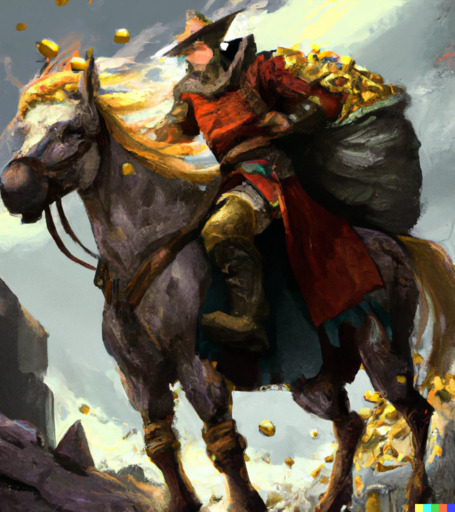
\includegraphics[width=\columnwidth]{equipment/tools goods and mounts}

    The world of Rise has a wide range of minor items like backpacks, blankets, and ten-foot poles.
    In general, the cost of those items is so insignificant from the perspective of an adventuring party that it's not worth the effort to track their cost in detail.
    A subset of particularly expensive items is included in \tref{Consumable Tools} and \tref{Permanent Tools, Goods, and Mounts}.

    \subsection{Standard Adventuring Kit}
        % Technically 15.2 gp and 50.5 pounds
        A standard adventuring kit costs 10 gp, weighs 50 pounds, and contains the following items:
        \begin{itemize}
            \item Backpack
            \item Bedroll
            \item Flint and steel
            \item Rations, trail (8 days)
            \item Rope, hempen (60 ft.)
            \item Sack (empty)
            \item Tent
            \item Torch
            \item Waterskin
        \end{itemize}

    
\begin{longtabuwrapper}
\begin{longtabu}{l l l X l}
\lcaption{Tool Items} \\
\tb{Name} & \tb{Level} & \tb{Typical Price} & \tb{Description} & \tb{Page} \tableheaderrule
Acid Flask & 1/2 & 2 gp & Throw to deal acid damage & \pageref{item:Acid Flask} \\
Alchemist's Fire & 1/2 & 2 gp & Throw to deal fire damage & \pageref{item:Alchemist's Fire} \\
Flash Powder & 1/2 & 2 gp & Emits burst of bright light & \pageref{item:Flash Powder} \\
Tindertwig & 1/2 & 2 gp & Quickly activated flame & \pageref{item:Tindertwig} \\
Potion of Wound Closure & \nth{1} & 10 gp & Grants \plus1 bonus to a \glossterm{wound roll} & \pageref{item:Potion of Wound Closure} \\
Smokestick & \nth{1} & 10 gp & Creates a cloud of smoke & \pageref{item:Smokestick} \\
Everburning Torch & \nth{3} & 50 gp & Emits light like a torch for a week & \pageref{item:Everburning Torch} \\
Potion of Healing & \nth{3} & 50 gp & Restores one hit point & \pageref{item:Potion of Healing} \\
Snowball & \nth{3} & 50 gp & Throw to deal cold damage & \pageref{item:Snowball} \\
Sunrod & \nth{3} & 50 gp & Emits bright light continuously & \pageref{item:Sunrod} \\
Tanglefoot Bag & \nth{3} & 50 gp & Slows a foe & \pageref{item:Tanglefoot Bag} \\
Thunderstone & \nth{3} & 50 gp & Deafens a foe & \pageref{item:Thunderstone} \\
Antitoxin Elixir & \nth{4} & 100 gp & Resists poisons & \pageref{item:Antitoxin Elixir} \\
Enduring Sunrod & \nth{6} & 240 gp & Emits bright light continuously & \pageref{item:Enduring Sunrod} \\
Enduring Antitoxin Elixir & \nth{7} & 360 gp & Resists poisons for 8 hours & \pageref{item:Enduring Antitoxin Elixir} \\
Potion of Wound Closure, Greater & \nth{7} & 360 gp & Grants \plus2 bonus to a \glossterm{wound roll} & \pageref{item:Potion of Wound Closure, Greater} \\
Potion of Healing, Greater & \nth{9} & 800 gp & Restores two hit points & \pageref{item:Potion of Healing, Greater} \\
Cleansing Potion & \nth{11} & 2,000 gp & Removes a condition & \pageref{item:Cleansing Potion} \\
Potion of Wound Closure, Supreme & \nth{13} & 5,000 gp & Grants \plus3 bonus to a \glossterm{wound roll} & \pageref{item:Potion of Wound Closure, Supreme} \\
Potion of Healing, Supreme & \nth{15} & 11,000  gp & Restores three hit points & \pageref{item:Potion of Healing, Supreme} \\
Cleansing Potion, Greater & \nth{17} & 25,000 gp & Removes two conditions & \pageref{item:Cleansing Potion, Greater} \\
\end{longtabu}
\end{longtabuwrapper}


    
\lowercase{\hypertarget{item:Potion (1st)}{}}\label{item:Potion (1st)}
\hypertarget{item:Potion (1st)}{\subsubsection{Potion (1st)\hfill1/2 (10 gp)}}

This potion contains the power of a 1st level \glossterm{targeted} spell that does not have the \glossterm{Attune} or \glossterm{Sustain} tags.
As a \glossterm{standard action}, you can spend an \glossterm{action point} to drink this potion.
When you do, if your \glossterm{power} is at least as high as this item's \glossterm{power}, the spell takes effect on you.
You are the only target of the spell.
If your \glossterm{power} is less than the item's \glossterm{power}, the overwhelming magical energy instead deals \glossterm{standard damage} \minus1d to you.

After this potion has been used, its magic is expended.



\parhead*{Materials} Alchemy


\lowercase{\hypertarget{item:Potion (2nd)}{}}\label{item:Potion (2nd)}
\hypertarget{item:Potion (2nd)}{\subsubsection{Potion (2nd)\hfill\nth{1} (50 gp)}}

This item functions like a 1st level potion, except that it contains a 2nd level spell.



\parhead*{Materials} Alchemy


\lowercase{\hypertarget{item:Potion (3rd)}{}}\label{item:Potion (3rd)}
\hypertarget{item:Potion (3rd)}{\subsubsection{Potion (3rd)\hfill\nth{4} (500 gp)}}

This item functions like a 1st level potion, except that it contains a 3rd level spell.



\parhead*{Materials} Alchemy


\lowercase{\hypertarget{item:Potion (4th)}{}}\label{item:Potion (4th)}
\hypertarget{item:Potion (4th)}{\subsubsection{Potion (4th)\hfill\nth{7} (1,800 gp)}}

This item functions like a 1st level potion, except that it contains a 4th level spell.



\parhead*{Materials} Alchemy


\lowercase{\hypertarget{item:Potion (5th)}{}}\label{item:Potion (5th)}
\hypertarget{item:Potion (5th)}{\subsubsection{Potion (5th)\hfill\nth{10} (6,500 gp)}}

This item functions like a 1st level potion, except that it contains a 5th level spell.



\parhead*{Materials} Alchemy


\lowercase{\hypertarget{item:Potion (6th)}{}}\label{item:Potion (6th)}
\hypertarget{item:Potion (6th)}{\subsubsection{Potion (6th)\hfill\nth{13} (25,000 gp)}}

This item functions like a 1st level potion, except that it contains a 6th level spell.



\parhead*{Materials} Alchemy

